% Options for packages loaded elsewhere
% Options for packages loaded elsewhere
\PassOptionsToPackage{unicode}{hyperref}
\PassOptionsToPackage{hyphens}{url}
%
\documentclass[
  4pt,
]{report}
\usepackage{xcolor}
\usepackage[paperheight=22.5cm,paperwidth=17cm]{geometry}
\usepackage{amsmath,amssymb}
\setcounter{secnumdepth}{3}
\usepackage{iftex}
\ifPDFTeX
  \usepackage[T1]{fontenc}
  \usepackage[utf8]{inputenc}
  \usepackage{textcomp} % provide euro and other symbols
\else % if luatex or xetex
  \usepackage{unicode-math} % this also loads fontspec
  \defaultfontfeatures{Scale=MatchLowercase}
  \defaultfontfeatures[\rmfamily]{Ligatures=TeX,Scale=1}
\fi
\usepackage[]{libertinus}
\ifPDFTeX\else
  % xetex/luatex font selection
\fi
% Use upquote if available, for straight quotes in verbatim environments
\IfFileExists{upquote.sty}{\usepackage{upquote}}{}
\IfFileExists{microtype.sty}{% use microtype if available
  \usepackage[]{microtype}
  \UseMicrotypeSet[protrusion]{basicmath} % disable protrusion for tt fonts
}{}
\usepackage{setspace}
\makeatletter
\@ifundefined{KOMAClassName}{% if non-KOMA class
  \IfFileExists{parskip.sty}{%
    \usepackage{parskip}
  }{% else
    \setlength{\parindent}{0pt}
    \setlength{\parskip}{6pt plus 2pt minus 1pt}}
}{% if KOMA class
  \KOMAoptions{parskip=half}}
\makeatother
% Make \paragraph and \subparagraph free-standing
\makeatletter
\ifx\paragraph\undefined\else
  \let\oldparagraph\paragraph
  \renewcommand{\paragraph}{
    \@ifstar
      \xxxParagraphStar
      \xxxParagraphNoStar
  }
  \newcommand{\xxxParagraphStar}[1]{\oldparagraph*{#1}\mbox{}}
  \newcommand{\xxxParagraphNoStar}[1]{\oldparagraph{#1}\mbox{}}
\fi
\ifx\subparagraph\undefined\else
  \let\oldsubparagraph\subparagraph
  \renewcommand{\subparagraph}{
    \@ifstar
      \xxxSubParagraphStar
      \xxxSubParagraphNoStar
  }
  \newcommand{\xxxSubParagraphStar}[1]{\oldsubparagraph*{#1}\mbox{}}
  \newcommand{\xxxSubParagraphNoStar}[1]{\oldsubparagraph{#1}\mbox{}}
\fi
\makeatother


\usepackage{longtable,booktabs,array}
\usepackage{calc} % for calculating minipage widths
% Correct order of tables after \paragraph or \subparagraph
\usepackage{etoolbox}
\makeatletter
\patchcmd\longtable{\par}{\if@noskipsec\mbox{}\fi\par}{}{}
\makeatother
% Allow footnotes in longtable head/foot
\IfFileExists{footnotehyper.sty}{\usepackage{footnotehyper}}{\usepackage{footnote}}
\makesavenoteenv{longtable}
\usepackage{graphicx}
\makeatletter
\newsavebox\pandoc@box
\newcommand*\pandocbounded[1]{% scales image to fit in text height/width
  \sbox\pandoc@box{#1}%
  \Gscale@div\@tempa{\textheight}{\dimexpr\ht\pandoc@box+\dp\pandoc@box\relax}%
  \Gscale@div\@tempb{\linewidth}{\wd\pandoc@box}%
  \ifdim\@tempb\p@<\@tempa\p@\let\@tempa\@tempb\fi% select the smaller of both
  \ifdim\@tempa\p@<\p@\scalebox{\@tempa}{\usebox\pandoc@box}%
  \else\usebox{\pandoc@box}%
  \fi%
}
% Set default figure placement to htbp
\def\fps@figure{htbp}
\makeatother


% definitions for citeproc citations
\NewDocumentCommand\citeproctext{}{}
\NewDocumentCommand\citeproc{mm}{%
  \begingroup\def\citeproctext{#2}\cite{#1}\endgroup}
\makeatletter
 % allow citations to break across lines
 \let\@cite@ofmt\@firstofone
 % avoid brackets around text for \cite:
 \def\@biblabel#1{}
 \def\@cite#1#2{{#1\if@tempswa , #2\fi}}
\makeatother
\newlength{\cslhangindent}
\setlength{\cslhangindent}{1.5em}
\newlength{\csllabelwidth}
\setlength{\csllabelwidth}{3em}
\newenvironment{CSLReferences}[2] % #1 hanging-indent, #2 entry-spacing
 {\begin{list}{}{%
  \setlength{\itemindent}{0pt}
  \setlength{\leftmargin}{0pt}
  \setlength{\parsep}{0pt}
  % turn on hanging indent if param 1 is 1
  \ifodd #1
   \setlength{\leftmargin}{\cslhangindent}
   \setlength{\itemindent}{-1\cslhangindent}
  \fi
  % set entry spacing
  \setlength{\itemsep}{#2\baselineskip}}}
 {\end{list}}
\usepackage{calc}
\newcommand{\CSLBlock}[1]{\hfill\break\parbox[t]{\linewidth}{\strut\ignorespaces#1\strut}}
\newcommand{\CSLLeftMargin}[1]{\parbox[t]{\csllabelwidth}{\strut#1\strut}}
\newcommand{\CSLRightInline}[1]{\parbox[t]{\linewidth - \csllabelwidth}{\strut#1\strut}}
\newcommand{\CSLIndent}[1]{\hspace{\cslhangindent}#1}



\setlength{\emergencystretch}{3em} % prevent overfull lines

\providecommand{\tightlist}{%
  \setlength{\itemsep}{0pt}\setlength{\parskip}{0pt}}



 


\usepackage{booktabs}
\usepackage{longtable}
\usepackage{array}
\usepackage{multirow}
\usepackage{wrapfig}
\usepackage{float}
\usepackage{colortbl}
\usepackage{pdflscape}
\usepackage{tabu}
\usepackage{threeparttable}
\usepackage{threeparttablex}
\usepackage[normalem]{ulem}
\usepackage{makecell}
\usepackage{xcolor}
\usepackage{siunitx}

    \newcolumntype{d}{S[
      table-align-text-before=false,
      table-align-text-after=false,
      input-symbols={-,\*+()}
    ]}
  
\usepackage{lscape}
\newcommand{\blandscape}{\begin{landscape}}
\newcommand{\elandscape}{\end{landscape}}
\usepackage{amsmath}
\makeatletter
\@ifpackageloaded{caption}{}{\usepackage{caption}}
\AtBeginDocument{%
\ifdefined\contentsname
  \renewcommand*\contentsname{Table of contents}
\else
  \newcommand\contentsname{Table of contents}
\fi
\ifdefined\listfigurename
  \renewcommand*\listfigurename{List of Figures}
\else
  \newcommand\listfigurename{List of Figures}
\fi
\ifdefined\listtablename
  \renewcommand*\listtablename{List of Tables}
\else
  \newcommand\listtablename{List of Tables}
\fi
\ifdefined\figurename
  \renewcommand*\figurename{Figure}
\else
  \newcommand\figurename{Figure}
\fi
\ifdefined\tablename
  \renewcommand*\tablename{Table}
\else
  \newcommand\tablename{Table}
\fi
}
\@ifpackageloaded{float}{}{\usepackage{float}}
\floatstyle{ruled}
\@ifundefined{c@chapter}{\newfloat{codelisting}{h}{lop}}{\newfloat{codelisting}{h}{lop}[chapter]}
\floatname{codelisting}{Listing}
\newcommand*\listoflistings{\listof{codelisting}{List of Listings}}
\makeatother
\makeatletter
\makeatother
\makeatletter
\@ifpackageloaded{caption}{}{\usepackage{caption}}
\@ifpackageloaded{subcaption}{}{\usepackage{subcaption}}
\makeatother
\usepackage{bookmark}
\IfFileExists{xurl.sty}{\usepackage{xurl}}{} % add URL line breaks if available
\urlstyle{same}
\hypersetup{
  hidelinks,
  pdfcreator={LaTeX via pandoc}}


\author{}
\date{August 11, 2025}
\begin{document}

\renewcommand*\contentsname{Table of contents}
{
\setcounter{tocdepth}{1}
\tableofcontents
}
\listoffigures
\listoftables

\setstretch{1.25}
\chapter*{Introduction}\label{introduction}
\addcontentsline{toc}{chapter}{Introduction}

Job loss can cause severe income disruptions, yet in the absence of
public intervention, workers must self-insure by borrowing, drawing down
savings, or relying on informal support networks. Economists have long
argued that such self-insurance is inefficient: when credit markets are
incomplete and workers are risk-averse, precautionary strategies often
fall short, and the welfare losses from income volatility can be large.
Unemployment insurance (UI) programs address this market failure by
pooling risk across individuals and time, thereby enabling workers to
smooth consumption during periods of joblessness
(\citeproc{ref-baily1978}{Baily 1978}; \citeproc{ref-gruber1997}{Gruber
1997}). Beyond their insurance function, UI programs may also improve
job match quality by reducing the urgency to accept the first available
job, leading to higher earnings and long-run productivity
(\citeproc{ref-acemoglu1999}{Acemoglu and Shimer 1999},
\citeproc{ref-acemoglu2000}{2000}).

These benefits, however, must be balanced against potential moral
hazard; generous benefits may reduce the urgency to search for work,
prolonging unemployment. In developing countries, where fiscal capacity
is limited and informality widespread, traditional UI systems are often
unviable. As a result, many governments rely on self-financed
alternatives designed to provide limited liquidity while minimizing work
disincentives. One such program is Mexico's \emph{Retiro Parcial por
Desempleo} (RPD), which allows unemployed formal-sector workers to
withdraw a portion of their pension savings upon job loss.

This paper addresses the question: What are the causal labor market
effects of access to the RPD program in Mexico? I study the impact of
RPD eligibility and take-up on three key outcomes: (i) job search
behavior, proxied by unemployment duration and employment survival; (ii)
job quality, measured by reemployment wages and job duration; and (iii)
medium-term labor market performance, defined as formal earnings and
months worked in the three years following displacement. Understanding
these effects is critical for assessing whether quasi-UI schemes like
RPD enable better job matches or merely delay reemployment, and whether
they reinforce or mitigate longer-term income risks.

A growing body of research has examined the effects of UI on labor
market outcomes in both high- and low-income contexts. In advanced
economies, natural experiments and regression discontinuity designs show
that more generous UI consistently prolongs unemployment spells (e.g.,
\citeproc{ref-katz1990}{Katz and Meyer 1990};
\citeproc{ref-schmieder2012}{Schmieder, Wachter, and Bender 2012}).
Evidence on job quality is more mixed: while some studies report gains
in reemployment wages and job stability (e.g.,
\citeproc{ref-nekoei2017}{Nekoei and Weber 2017};
\citeproc{ref-centeno2006}{Centeno and Novo 2006}), others find
negligible or even adverse effects on earnings (e.g.,
\citeproc{ref-schmieder2016}{Schmieder and Wachter 2016};
\citeproc{ref-lebarbanchon2016}{Le Barbanchon 2016}). In middle-income
countries, UI interacts with informality in complex ways. For instance,
Britto (\citeproc{ref-britto2022}{2022}) finds that in Brazil, over half
of the additional unemployment induced by extended UI is offset by
increased informal employment, raising concerns about behavioral leakage
and program effectiveness.

This study contributes to the literature by being the first to estimate
the causal impact of Mexico's RPD program using administrative data and
a fuzzy regression discontinuity design. While earlier causal studies
(e.g., \citeproc{ref-veluxe1zquezguadarrama2023}{Velázquez Guadarrama
2023}; \citeproc{ref-carreuxf1ogoduxednez2025}{Carreño Godínez 2025})
relied on survey data, I leverage high-frequency longitudinal records
from the Mexican social security system to construct a clean analytic
sample and directly observe eligibility, take-up, and formal labor
market trajectories. The RPD's eligibility threshold---requiring at
least two years of social security contributions---offers a compelling
quasi-experimental setting. By exploiting this discontinuity and
tracking administrative take-up, I estimate local average treatment
effects (LATEs) for compliers across a rich set of labor market
outcomes. While internal validity is strong, generalizability is limited
to younger formal-sector workers near the eligibility threshold.

The results show that RPD take-up has large and significant effects on
unemployment duration: users remain unemployed for approximately 36
additional weeks over a three-year period, from a baseline of 51 weeks
for the ineligible, with effects evident within the first three months
after displacement. However, these extended unemployment spells do not
translate into higher job quality. On average, RPD users do not
experience gains in wages, job duration, or cumulative earnings. In
fact, most subgroups---particularly lower-income, younger, and female
workers---experience substantial earnings losses over the three-year
horizon. Although some subgroups, such as higher-income or male workers,
see small gains in reemployment earnings, these are not sufficient to
offset longer unemployment spells. These findings challenge optimistic
models of UI that predict gains in productivity and matching quality
(\citeproc{ref-acemoglu2000}{Acemoglu and Shimer 2000}), and instead
suggest that self-financed programs like RPD may distort job search
without delivering meaningful returns in terms of labor market outcomes.

Importantly, heterogeneity analyses reveal that the effects of RPD vary
markedly across demographic and macroeconomic conditions. Younger and
lower-wage workers face much larger increases in unemployment and
sharper earnings losses---suggesting that RPD may exacerbate, rather
than alleviate, pre-existing vulnerabilities, and thus renforce
inequality. In contrast, workers displaced during the COVID-19 crisis
exhibit smaller increases in unemployment and even experience modest
gains in cumulative earnings. This points to a potentially
countercyclical role for liquidity provision, where temporary support
during downturns may cushion income losses and facilitate labor market
reintegration.

These findings offer several policy-relevant insights. First, the
structure of the RPD program; being self-financed and actuarially
neutral---appears to reduce concerns about fraud and fiscal burden but
also limits its redistributive potential. Second, the regressive nature
of its benefits---favoring those with more savings and stronger labor
market histories---raises concerns about equity and adequacy. Lastly,
while the program may be appropriate as a minimal safety net, it does
not substitute for the functions of traditional unemployment insurance.
The results contribute empirical grounding to policy debates in Mexico
and other developing economies over whether to expand self-financed
schemes, replace them with publicly funded UI, or design hybrid systems
tailored to institutional capacity.

Nonetheless, the study has limitations. The fuzzy RD design identifies
local treatment effects for a narrow group of workers---those displaced
in their third year of formal labor market participation---limiting
external validity. Moreover, the administrative data do not capture
transitions into informal employment or broader welfare outcomes, such
as psychological stress or household income dynamics. Finally, the
modest first stage---only a 4 percentage point increase in
take-up---constrains precision in second-stage estimates and
necessitates cautious interpretation.

The remainder of the paper proceeds as follows.
Section~\ref{sec-lit-review} reviews the literature on UI and quasi-UI
programs in both developed and developing countries.
Section~\ref{sec-context} provides institutional background on the RPD
program and Mexico's broader unemployment protection framework.
Section~\ref{sec-data} describes the data and sample construction.
Section~\ref{sec-empirical-strategy} outlines the empirical strategy.
Section~\ref{sec-results} presents the main results, including
heterogeneity analysis. I finish with a discussion of the findings and
their implications for policy.

\chapter{Literature Review}\label{sec-lit-review}

This section reviews key strands of the unemployment protection
literature relevant to the Retiro Parcial por Desempleo (RPD). I begin
by outlining the evolution of economic thought on unemployment insurance
(UI), followed by empirical evidence on its labor market effects. I then
examine how UI functions in developing economies, where informality and
weak enforcement complicate its impact. Finally, I turn to
pension-linked and quasi-UI schemes, focusing on RPD as a self-financed
alternative in a context with limited access to formal unemployment
support.

\section{History of Economic Thought on Unemployment
Insurance}\label{history-of-economic-thought-on-unemployment-insurance}

Unemployment insurance (UI) has its roots in early 20th-century social
insurance schemes, introduced to buffer workers against income loss
during joblessness. Economists and policymakers initially debated its
merits: while UI promised to stabilize incomes and aggregate demand
(especially during downturns like the Great Depression), critics warned
even early on that providing benefits to the unemployed could weaken
work incentives (\citeproc{ref-price1985}{Price 1985}).

Over time, UI became a standard component of the welfare state -- by
1935 the U.S. had a federal-state UI system, following earlier European
models -- and was seen as both a social safety net and an automatic
stabilizer for the economy. Classic economic thought began formalizing
this trade-off in the 1960s and 1970s. For example, job search theory
highlighted that more generous UI would raise workers' reservation wages
and reduce search intensity, potentially lengthening unemployment spells
(\citeproc{ref-stigler1961}{Stigler 1961},
\citeproc{ref-stigler1962}{1962}).

By the late 1970s, seminal theoretical contributions articulated the
balance between consumption smoothing benefits and moral hazard costs of
UI. Baily (\citeproc{ref-baily1978}{1978}) derived the optimal benefit
replacement rate under this trade-off, showing that while risk-averse
workers gain welfare from smoothing consumption during unemployment, too
generous a benefit can induce longer spells of joblessness. Subsequent
models, such as Shavell and Weiss (\citeproc{ref-shavell1979}{1979})
explored optimal time profiles of benefits, suggesting payments should
ideally decline over the spell to encourage re-employment. These early
theories formalized the notion that UI's insurance value must be weighed
against incentive effects.

Empirically, evidence soon confirmed UI's consumption-smoothing role:
Gruber (\citeproc{ref-gruber1997}{1997}) found that a 10
percentage-point increase in the UI replacement rate reduces the drop in
household consumption on job loss by about 2.7\%, significantly
cushioning unemployed families. This finding provided quantitative
support for the idea that UI mitigates welfare losses during
unemployment. At the same time, researchers noted that UI could raise
unemployment rates. Katz and Meyer (\citeproc{ref-katz1990}{1990}) used
administrative data to show that a one week increase of UI benefit
duration increases the average unemployment duration by 0.16 to 0.20
weeks. Thus, by the 1990s, the economics literature broadly accepted
that UI entails a trade-off: it protects income and consumption for the
unemployed, but creates moral hazard that can aggravate unemployment.

Importantly, later theoretical work added nuance to this view. General
equilibrium and job-matching models indicated that UI might improve the
quality of job matches. For instance, Acemoglu and Shimer
(\citeproc{ref-acemoglu2000}{2000}) argued that more generous UI could
lead workers to seek higher-productivity jobs, potentially raising
long-run output. Others pointed out that UI's effect on job-finding
could be offset by better matches or higher post-unemployment wages.
Over the decades, UI became a focal example of optimal policy design
under uncertainty: Hopenhayn and Nicolini
(\citeproc{ref-hopenhayn1997}{1997}) derived formulas for an ideal UI
system that gradually decreases benefits to incent re-employment, and
later ``sufficient statistics'' approaches (e.g. Chetty
(\citeproc{ref-chetty2008}{2008})) quantified the welfare trade-off
using risk aversion and behavioral elasticities.

By the 2000s, surveys of the literature (Atkinson and Micklewright
(\citeproc{ref-atkinson1991}{1991}); Krueger and Meyer
(\citeproc{ref-krueger2002}{2002})) concluded that while UI undoubtedly
prolongs unemployment spells, it also substantially raises recipients'
welfare by smoothing consumption and can even yield positive
externalities (like better job matches or macroeconomic stabilization).
A recent meta-analysis of 55 studies reinforces this historical
perspective: it finds that despite some publication bias inflating
earlier estimates, UI benefits do have a tangible ``disemployment''
effect (elasticity of unemployment duration with respect to benefit
generosity on the order of 0.2--0.5) -- yet an optimal policy is not
zero UI, rather a moderate replacement rate around 30\% is
welfare-maximizing once both insurance and behavioral responses are
accounted for (\citeproc{ref-cohen2024}{Cohen and Ganong 2024}). In
summary, the evolution of economic thought on UI has progressed from
simple cautionary tales about work disincentives to a sophisticated
understanding of how UI can be designed to balance equity and efficiency
over the business cycle.

\section{Empirical Evidence}\label{empirical-evidence}

A large empirical literature, especially from the 1980s onward, has
quantified the labor market effects of unemployment insurance. Early
empirical studies used aggregate time-series or cross-sectional
variation and found suggestive correlations between generous UI and
higher unemployment. However, more rigorous evidence emerged as
researchers exploited policy changes and micro-data. The landmark study
by Katz and Meyer (\citeproc{ref-katz1990}{1990}) demonstrated a sharp
spike in the job-finding rate as unemployed workers' benefits were about
to expire, indicating that many workers remained unemployed until their
UI ran out and then quickly found jobs. This provided clear evidence
that UI availability lengthens unemployment spells. Around the same
time, Meyer (\citeproc{ref-meyer1990}{1990}) estimated that higher
benefit levels or longer entitlement durations significantly reduce the
hazard rate of leaving unemployment, with implied elasticities often in
the range of 0.4--0.6. In practical terms, a 10\% increase in the UI
benefit level was found to increase average unemployment durations by
roughly 4--8\% in the U.S. context (Krueger and Meyer
(\citeproc{ref-krueger2002}{2002})). Such findings, replicated in Canada
and Europe, solidified the consensus that more generous UI leads to
longer spells of insured unemployment, all else equal.

Notably, this effect was not merely observational -- it was confirmed by
natural experiments. For example, when the U.S. extended benefit
durations during recessions, researchers observed proportional increases
in unemployment length (\citeproc{ref-moffitt1985}{Moffitt 1985}).
Similarly, Lalive (\citeproc{ref-lalive2008}{2008}) examined an Austrian
program that dramatically extended benefits for older workers (from 1
year to up to 4 years) and found the job-finding rate plummeted for the
treated group. In essence, as benefits became available for longer,
workers -- especially those near retirement age -- delayed re-entry into
employment. These seminal contributions established a causal link
between UI and labor supply behavior, leveraging
difference-in-differences (policy reforms across regions or time) and
regression discontinuity designs for credible identification.

Over time, researchers applied increasingly creative strategies to pin
down causality. Regression discontinuity (RD) designs have been
particularly influential. In some countries, UI benefit schedules or
durations change discontinuously with age or tenure. Schmieder, Wachter,
and Bender (\citeproc{ref-schmieder2012}{2012}) exploited age thresholds
in Germany's UI system and confirmed that extending UI entitlement by
one month causally increases unemployment duration (by roughly 0.1--0.2
months on average), remarkably similar to estimates from the U.S. and
elsewhere. Likewise, Lalive (\citeproc{ref-lalive2007}{2007}) and Card,
Chetty, and Weber (\citeproc{ref-card2007}{2007}) used RD and related
methods in Austria and found sizable effects on spell length when
benefits were extended. The consistency of findings across settings
(U.S., Canada, Europe) lent credibility to the external validity of the
result: UI dampens the urgency of job search.

In addition, randomized experiments have been conducted to study UI
incentives. One famous trial was the Illinois Reemployment Bonus
Experiment in the 1980s, which offered UI recipients a lump-sum bonus
for quick reemployment. The experiment showed that modest financial
incentives (\$500 bonuses) induced earlier exits from unemployment,
albeit the effects were not large (e.g.~reducing average duration by
about a week) and the program's cost-effectiveness was debated.
Nonetheless, it confirmed that unemployed workers respond to financial
incentives, reinforcing the evidence that the structure of UI benefits
influences behavior.

Beyond unemployment duration, seminal studies have examined how UI
affects other labor market outcomes like re-employment wages, job match
quality, and long-run earnings. Theoretically, longer search enabled by
UI could lead to better matches (higher wages or productivity), but
longer non-employment could also erode skills or signal lower
productivity to employers. The empirical evidence is mixed. On the one
hand, several studies find positive effects on job quality: for example,
a recent study in Austria found that a moderate extension of benefits
led to a 0.5\% increase in re-employment wages on average
(\citeproc{ref-nekoei2017}{Nekoei and Weber 2017}), suggesting that
extra search time helped workers find better matches. And in the United
States, longer potential UI durations have been linked to unemployed
individuals holding out for higher productivity jobs, which can even
spur job creation by improving matching efficiency
(\citeproc{ref-centeno2006}{Centeno and Novo 2006}). These findings echo
the insight of Acemoglu and Shimer (\citeproc{ref-acemoglu2000}{2000})
that UI can raise overall productivity.

On the other hand, some research finds little gain in match quality: a
study in Germany found a slight reduction in re-employment wages
(\textasciitilde0.8\%) when benefits were extended
(\citeproc{ref-schmieder2016}{Schmieder and Wachter 2016}) and a study
in France detected no discernible impact on subsequent job match quality
or wages (\citeproc{ref-lebarbanchon2016}{Le Barbanchon 2016}). Thus,
while UI unambiguously lengthens unemployment spells, its impact on
post-unemployment outcomes can vary -- with some contexts showing
improved job matches and others showing flat or slightly negative
effects. Part of this difference may arise from whether UI mainly delays
acceptance of \emph{sub-par} jobs (thereby improving matches) or whether
it causes skill atrophy. Recent meta-analyses and cross-country
comparisons indicate that in aggregate, the micro-elasticity of
unemployment with respect to UI is similar to the macro-level impact,
implying that general equilibrium effects (like wage adjustments or
vacancy creation) do not dramatically alter the basic conclusion
(\citeproc{ref-cohen2024}{Cohen and Ganong 2024}). In summary, the
seminal empirical literature -- through a combination of natural
experiments, policy discontinuities, and even randomized trials -- has
firmly established that UI benefits \emph{cause} longer unemployment
spells, while also highlighting important nuances in terms of search
intensity, job quality, and the optimal calibration of UI in different
contexts.

\section{Developing Countries and Informal Labor
Markets}\label{developing-countries-and-informal-labor-markets}

While most classic UI studies focus on advanced economies, a growing
body of research examines how unemployment benefits operate in
developing countries, where labor markets are characterized by high
informality and weaker administrative capacity (\citeproc{ref-ulku}{Ulku
and Georgieva, n.d.}). In many developing economies, formal UI systems
either did not exist historically or covered only a small fraction of
workers. Instead, governments often relied on protective labor
regulations -- such as stringent job security rules and mandated
severance pay -- as a way to shield workers from income loss. This
``protecting jobs'' approach (e.g.~requiring large severance payouts or
restricting layoffs) was seen as more feasible in environments without
the bureaucratic means to implement a contributory UI system. However,
it came at the cost of labor market rigidity
(\citeproc{ref-garibaldi2005}{Garibaldi and Violante 2005}). By the
2000s, there was increasing recognition that overly strict labor
regulations impeded job creation, leading to reforms embracing
``flexicurity'' -- flexibility in hiring/firing combined with security
via unemployment benefits. Chile's introduction of a national UI system
in 2002 was a pioneering example, and other middle-income countries
(Brazil, Colombia, etc.) gradually expanded or created UI programs. Yet,
implementing UI in developing contexts raises unique challenges: most
notably, the presence of a large informal sector where workers and firms
operate outside the regulated, tax-paying economy.

A key question is how informal labor markets interact with unemployment
insurance. Conventional wisdom suggested that UI could be especially
distortionary in such settings -- for example, workers might continue
working informally while claiming UI, effectively turning the benefit
into a hidden subsidy for off-the-books employment. Indeed, early
analyses posited that a large informal sector would magnify UI's moral
hazard problem, as beneficiaries could earn untaxed income without
forfeiting benefits (\citeproc{ref-hartley2011}{Hartley, Ours, and
Vodopivec 2011}). Recent research has sought to quantify these effects.
In an important study on Brazil, Gerard and Gonzaga
(\citeproc{ref-gerard2021}{2021}) combined an optimal UI framework with
Brazilian data to evaluate whether informality increases the efficiency
costs of UI. Using a quasi-experimental variation in benefit duration
(an age-based eligibility cutoff for extended benefits), they found the
usual result that UI prolongs formal unemployment spells (moral hazard),
but intriguingly the efficiency cost was \emph{lower} in Brazil than in
the United States. In areas or demographic groups with higher
informality, the incremental effect of UI on formal re-employment was
smaller, essentially because formal job-finding rates were low to begin
with in those high-informality segments. Many workers would remain
jobless or informal with or without UI, so the relative ``excess''
duration caused by benefits was modest. Their conclusion was that moral
hazard may actually become a more salient concern as an economy
formalizes -- a counterintuitive insight that in very informal
economies, UI might do less harm than expected (since the alternative to
formal unemployment is often informal work or inactivity anyway).

Other evidence from developing countries, however, shows that UI can
induce shifts to informal employment during the insured spell. In
Brazil, formal employees are legally barred from concurrently holding a
registered job while on UI, but they can and often do find unregistered
work. Britto (\citeproc{ref-britto2022}{2022}) provides causal evidence
on this behavior. In his study of Brazil's UI system and severance pay
scheme (\emph{Fundo de Garantia do Tempo de Serviço}, FGTS), Britto
first uses a regression discontinuity design to show that receiving a
lump-sum severance payment (on formal job) lengthens the time until a
worker returns to a formal job by about 1.9 weeks after three years
since displacement. He then examines a one-month extension of UI
benefits (using another discontinuity in eligibility) and finds that the
extended UI causes an even larger initial increase in formal
unemployment duration compared to the lump-sum. Crucially, by matching
administrative data with household surveys, Britto finds that 57\% of
the ``lost'' formal employment time under extended UI is offset by
increased informal employment. In other words, more than half of those
extra weeks of formal joblessness are weeks in which the individuals are
working informally while collecting UI. This reveals a strategic
response: workers exploit the benefit by substituting formal jobs (which
would end UI receipt) with informal work until benefits are exhausted.
Such findings underscore the importance of informality as an auxiliary
unemployment insurance mechanism in developing economies.

That said, the medium-term impacts of UI in these contexts may be more
benign than the short-term behavior suggests. Britto's analysis shows
that although an extra month of UI induces a significant temporary drop
in formal employment, those on extended UI partially catch up in
employment after benefits expire, so that over a three-year horizon
their total time in formal work is similar to those who only got the
lump-sum. Moreover, the UI recipients found jobs with higher wages than
those who only got the lump-sum severance. This aligns with evidence
from other developing settings that UI can improve match quality or give
workers more bargaining power. Indeed, Britto finds the one-month UI
extension was less harmful to reemployment wages than the lump-sum
assistance, possibly because having ongoing benefits allowed workers to
hold out for better offers. Similarly, a study in Argentina found that
unemployment benefits recipients tended to find formal jobs with
slightly higher wages than non-recipients at only a moderate cost of
increased unemployment duration
(\citeproc{ref-gonzuxe1lez-rozada2023}{González-Rozada and Ruffo 2023}).

In summary, global evidence from middle- and low-income countries
suggests that the fundamental effects of UI -- consumption smoothing and
extended job-search time -- appear universal, but high informality
profoundly shapes outcomes. UI in developing economies often has
``leakage'' into the informal sector: some share of beneficiaries will
work outside the formal system while receiving benefits
(\citeproc{ref-britto2022}{Britto 2022}). This cushions their income (a
form of hidden employment) but undermines the intent of UI and raises
questions about monitoring. Yet, the presence of informality can also
mean the net social cost of UI is not as high as in a fully formal
setting, since many would not have formal jobs regardless
(\citeproc{ref-gerard2021}{Gerard and Gonzaga 2021}). Policymakers thus
face a dilemma: how to extend unemployment protection to workers in
economies where many do not work in the formal sector. Experiments are
ongoing -- for example, some countries have tested unemployment
assistance for self-employed or informal workers (often via cash
transfer programs rather than true ``insurance''). Overall, the
literature underscores that context matters -- the optimal design and
expected effects of UI in a developing country (with limited enforcement
and many informal jobs) will differ from those in a developed economy.
Research on Brazil, Mexico, Chile, and others is gradually filling in
these gaps, pointing to the importance of complementary policies (like
cracking down on informal work by UI claimants, integrating informal
workers into the system through incentives or through active labor
market policies) to make unemployment protection effective in the
developing world.

\section{Pension-Integrated and Quasi-UI
Schemes}\label{pension-integrated-and-quasi-ui-schemes}

Beyond traditional unemployment insurance, many countries have
implemented or experimented with alternative mechanisms to protect
workers against job loss. These \emph{pension-adjacent} or
\emph{quasi-UI} schemes include programs like lump-sum severance pay,
unemployment savings accounts, and allowing early withdrawals from
pension funds during unemployment. Such schemes are especially common in
countries that lack a comprehensive UI system or seek to reduce the
moral hazard associated with standard UI benefits.

Severance pay is the oldest and most widespread alternative to UI. Under
severance mandates, employers must provide a one-time payout to workers
upon involuntary separation, typically based on tenure. This lump-sum
acts as a form of unemployment compensation, but it is financed at the
firm level and paid only at layoff. Many Latin American and Asian
countries historically relied on severance pay in lieu of UI. However,
severance has well-documented shortcomings: it usually covers only
formal sector layoffs, provides no help to those who quit or were
informally employed, and may deter employers from hiring, or encourage
firing workers before they accumulate tenure.

Recognizing the limitations of pure severance pay, some countries have
adopted Unemployment Insurance Savings Accounts (UISAs) or hybrid
systems that combine self-insurance with social insurance. The idea of
UISAs, posited by academics like Feldstein and Altman
(\citeproc{ref-feldstein2007}{2007}), Orszag and Snower
(\citeproc{ref-orszag2002}{2002}) and Stiglitz and Yun
(\citeproc{ref-stiglitz2005}{2005}), is to have each worker accumulate
savings in an individual account during employment, which can be drawn
down during periods of unemployment. If the worker's account balance is
insufficient, a public solidarity fund or government backstop can cover
the difference, ensuring a minimum benefit, but importantly, any unused
balance remains the worker's property, often convertible to retirement
funds. This mechanism aims to \emph{internalize the cost} of
unemployment benefits -- since workers essentially pay for their own UI
(at least up to a point), they have less incentive to abuse the system.
In theory, UISAs should reduce the moral hazard problem inherent in
pooled UI, because any withdrawal today will deplete one's own savings
(or future pension), thereby discouraging unnecessary use.

Chile's UI system, introduced in 2002, is a flagship example of UISA. It
established individual unemployment accounts financed by payroll
contributions, alongside a common \emph{Fondo Solidario} for those who
exhaust their savings or have very low balances
(\citeproc{ref-hartley2011}{Hartley, Ours, and Vodopivec 2011}). Workers
first draw benefits from their personal account; only if that is empty
(and if they meet eligibility criteria) do they receive benefits from
the solidarity pool. This two-tier design was intended to preserve work
incentives while still providing a safety net for the most vulnerable.
By 2008, about 80\% of Chilean private-sector workers were contributing
to these accounts, and the system had expanded coverage dramatically
compared to the old severance pay regime.

Studies evaluating Chile's reform find encouraging results. Hartley,
Ours, and Vodopivec (\citeproc{ref-hartley2011}{2011}) reported that the
introduction of UISAs improved re-employment incentives: workers with
ample savings in their accounts did not prolong their unemployment
spells as much as they would have under a pure UI system, since they
were drawing on their own funds. In line with this, the authors found
that an extension of benefits financed by the solidarity fund led to
longer unemployment durations (a moral hazard effect), whereas those
relying solely on their individual accounts showed no increase in
unemployment duration. This absence of behavioral response in the
self-funded tier suggests that when workers use their own money
(forced-savings) for unemployment, they treat it differently than a
no-strings-attached benefit (\citeproc{ref-ulku}{Ulku and Georgieva,
n.d.}). Essentially, Chile's experience showed that moral hazard may be
sharply reduced by the UISA design -- a finding consistent with
theoretical expectations.

Following Chile, countries like Colombia and Mauritius implemented
similar savings-account-based unemployment benefit schemes
(\citeproc{ref-ulku}{Ulku and Georgieva, n.d.}). Colombia, for instance,
has a program of \emph{cesantías} (unemployment savings) where employers
deposit a month's pay per year into an account that workers can withdraw
upon separation or other contingencies. These systems blur the line
between pensions and unemployment insurance, effectively using a
pre-funded individual buffer to handle job-loss income shocks.

Mexico provides a salient case of a quasi-UI pension withdrawal scheme
with the \emph{Retiro Parcial por Desempleo} (RPD). Lacking a formal UI
program for most workers\footnote{A state-level unemployment insurance
  was implemented in Mexico City, albeit coverage is low, eligibility
  rules are obscure, and its benefits are small since it is funded
  through the state budget (\citeproc{ref-loaaguirre2019}{Loa Aguirre
  and Rubio Campos 2019}).}, Mexico allows individuals to make a
withdrawal from their Afore (individual retirement savings account) when
they become unemployed. This policy, in effect since the early 2000s,
treats the retirement account as a self-insurance vehicle for
unemployment.\footnote{I present the features of the RPD program in
  detail in Section~\ref{sec-context}.} Studies by Mexico's pension
regulator have noted a sharp increase in such withdrawals, especially
during the COVID-19 Pandemic, and have continued to raise since
(\citeproc{ref-consar2024}{CONSAR 2024}), likely due to the increased
salience that the program achieved during the employment crisis that
followed the COVID-19 pandemic.

Empirical evidence of the RPD scheme is still emerging. One concern is
that allowing easy access to pension funds in mid-career could undermine
long-term savings adequacy. Another is that, similar to severance, a
one-off withdrawal may be spent quickly. Evidence from Brazil's
severance suggests people exhibit \emph{present bias}: Gerard and
Naritomi (\citeproc{ref-gerard2021a}{2021}) showed that upon layoff,
Brazilian workers who received their FGTS lump-sum increased their
consumption by 35\% in the initial weeks, even though they subsequently
faced a 14\% drop in consumption in the longer term. This indicates that
lump-sum payments tend to be consumed rather than smoothed, potentially
leaving individuals unprotected later in their unemployment spell. We
might expect a similar pattern for pension withdrawals -- an upfront
infusion that could be exhausted before re-employment, thereby failing
to fully smooth income over the unemployment duration.

Velázquez Guadarrama (\citeproc{ref-veluxe1zquezguadarrama2023}{2023})
used public data from the \emph{Encuesta Nacional de Ocupación y Empleo}
(ENOE) and a regression discontinuity design to show that the RPD
program has several significant causal effects on labor market outcomes.
Specifically, the study estimates that being eligible for the RPD
increases salary income by 2.47\%, suggesting that having access to
these funds allows individuals to pursue potentially riskier,
better-paying jobs or engage in longer hiring processes. He also finds
that eligibility increases the probability of being employed by 2.67\%,
a result noted as potentially counterintuitive, but which might be
explained by individuals taking jobs perceived as having a higher risk
of future unemployment or, importantly, demonstrating that the moral
hazard often associated with traditional unemployment insurance is
mitigated since the funds are drawn from the individual's own savings.
Finally, eligibility leads to an estimated increase in the duration of
unemployment by 83 days, implying that individuals eligible for the
program utilize the financial support to extend their job search and
find a better match for their skills and needs. These results
collectively suggest that integrating unemployment benefits with a
pension system, can be an effective mechanism for mitigating moral
hazard while potentially improving resource allocation in the labor
market through higher wages and employment probability, despite
increasing the duration of unemployment.

Moreover, Carreño Godínez
(\citeproc{ref-carreuxf1ogoduxednez2025}{2025}) also used ENOE data and
a Difference-in-Differences design to show that eligibility for the RPD
is estimated to increase the probability of transitioning into
entrepreneurship. Depending on the model specification used, this
increase is estimated to be between 5.01\% and 21.4\% greater for
eligible individuals compared to those who do not meet the eligibility
criteria. Carreño interprets these results as evidence that, in a
context like Mexico where access to credit is limited and a traditional
state-funded unemployment insurance does not exist, the early withdrawal
mechanism from individual retirement accounts (Afore) functions as a
financial safety net. This access to financial resources appears to
facilitate the creation of new businesses by providing individuals with
the necessary support to undertake the risky decision of starting an
enterprise. These findings suggest that mechanisms allowing access to
individual savings can indirectly promote entrepreneurship by providing
a lump-sum payment to the unemployed.

\chapter{Institutional Background}\label{sec-context}

This section provides an overview of the institutional framework
surrounding unemployment protection in Mexico, with a focus on the
\emph{Retiro Parcial por Desempleo} (RPD) program. I begin by describing
the eligibility conditions and usage rules of the RPD, a mechanism that
allows unemployed workers to make partial withdrawals from their
individual pension accounts. I then document the evolution of the
program's adoption over time, highlighting its increased relevance
during periods of economic crisis. Finally, I situate RPD within the
broader context of income substitution in Mexico, where the failure to
enforce legally mandated severance pay has rendered employer-based
protections largely ineffective. In this setting, RPD emerges as a
self-financed, readily accessible---but ultimately limited---alternative
for workers facing job loss.

\section{The Partial Withdrawal}\label{the-partial-withdrawal}

The RPD program works as follows. The pension system in Mexico is a
standard defined contributions scheme with individual accounts. While
working in formality, workers accumulate resources financed in part by
themselves, by their employer and by the government.

\subsection{Eligibility Criteria}\label{eligibility-criteria}

If a worker faces an unemployment spell of at least 46 days, she may
withdraw a fraction of her individual account balance through the RPD.
The amount of money a worker can have access to depends on the number of
years since her account was opened and the number of weeks she has
contributed to social security. The \emph{Ley del Seguro Social}
considers two eligibility schemes, each allowing a worker to withdraw an
amount up to:

\begin{enumerate}
\def\labelenumi{\Alph{enumi}.}
\item
  Ten months of the minimum wage or one month of her most recent wage,
  whichever is lower, for workers satisfying:

  \begin{enumerate}
  \def\labelenumii{\roman{enumii}.}
  \item
    having entered the formal labor market at least three years ago, and
  \item
    having contributed to social security for at least two
    years.\footnote{Contributions to social security need not be
      continuous to reach eligibility to RPD.}
  \end{enumerate}
\item
  Three times her monthly wage or 11.5\% of her account balance,
  whichever is lower, for workers who entered the formal labor market at
  least three years ago, regardless of contributions to social security.
\end{enumerate}

Figure~\ref{fig-eligibility} provides a visual representation of the
eligibility criteria. Note that a worker who became dismissed after four
years since she entered the labor market, and with only one year of
contributions to social security would not be immediately eligible to
withdraw funds from her account. However, if she just waited in
unemployment for a year, she would become eligible through Scheme B,
without having to make further contributions. Hence, ineligible workers
may become eligible by the mere passage of time. This feature of the
eligibility structure is important to the construction of the analysis
sample, as I show in Section~\ref{sec-sample-selection}.

Moreover, workers who are eligible through both schemes may choose the
one that allows them to withdraw the largest amount. Having used the RPD
once, a worker may use it again, only after waiting for five years since
her last withdrawal. Importantly, using the RPD not only depletes the
worker's individual pension savings account, but it also reduces
proportionally the amount of contributions to social security, which are
used to determine and finance the pension at retirement age. This is a
key feature of the RPD, as it allows workers to access their savings
during unemployment, but it also reduces their future pension benefits.

\begin{figure}

\caption{\label{fig-eligibility}Eligibility Criteria}

\centering{

\pandocbounded{\includegraphics[keepaspectratio]{thesis_files/figure-pdf/unnamed-chunk-1-1.pdf}}

\emph{Note:} This figure conceptualizes eligibility to RPD. The x-axis
shows the number of years since entry to the labor market, while the
y-axis shows the number of years contributed to social security. The
green area represents the eligibility criteria for Scheme A: having
entered the formal labor market at least three years before and having
contributed to social security for at lest two years. The blue area
represents the eligibility criteria for Scheme B: having entered the
formal labor market at least three years before, regardless of
contributions to social security. The gray area represents the not
feasible zone: workers cannot contribute more days to social security
than they have been in the formal labor market.

}

\end{figure}%

\section{Usage and Adoption}\label{sec-usage}

Figure~\ref{fig-rpd} shows the cumulative number of partial withdraws
from the individualized pension accounts since it was implemented in
1997. The data comes from a confidential administrative data set from
the \emph{Instituto Mexicano del Seguro Social} (IMSS). The RPD program
was first implement in 2009 to give unemployed workers a source of
income substitution in the context of the Great Recession. This event
can be seen as a sharp increase in the usage of RPD, but also as a
change in the trend of the number of withdrawals from the pension
system. Accordingly, in the next big employment crisis, the COVID-19
pandemic, another trend increase followed. This shifts in the slope of
the cumulative usage of RPD shows that employment crises have a
persistent effect on the usage of the program, likely due to the
increased salience of the program.

To put figures into perspective, by the end of 2024, 16,966,851 workers
had made 24,598,838 withdrawals from the pension system. By that same
moment, IMSS reported a total of 22,238,379 active workers in the formal
labor market. Indeed, not all RPD users were active workers by the end
of 2024, but this number gives a sense of the magnitude of the usage
program.

\begin{figure}

\caption{\label{fig-rpd}Usage and Adoption}

\centering{

\pandocbounded{\includegraphics[keepaspectratio]{thesis_files/figure-pdf/unnamed-chunk-3-1.pdf}}

\emph{Note:} This figure shows the cumulative number of partial
withdrawals (left) and the cumulative amount withdrawn (right) out of
the Mexican individual pension account system (Afore). Source: IMSS.

}

\end{figure}%

\section{Income Substitution for the Unemployed in
Mexico}\label{income-substitution-for-the-unemployed-in-mexico}

In theory, Mexican labor law provides mandatory severance pay
(indemnización constitucional) as the main form of income substitution
for workers who lose their jobs. Upon unjustified dismissal, employers
are required to provide affected workers with three months of salary,
plus seniority bonuses and accrued benefits. This legal severance
framework reflects the broader Latin American tradition of employer
liability systems as a substitute for unemployment insurance. However,
in practice, enforcement of these entitlements is weak, uneven, and
often illusory---rendering severance rights largely ineffective as a
tool for income smoothing during unemployment.

The core issue lies in the functioning of Mexico's labor courts. In
particular, in Mexico City, workers who wish to claim their legally
mandated severance must navigate a judicial process that is slow,
opaque, and vulnerable to both corruption and administrative
incompetence. Degetau (\citeproc{ref-degetau2023}{2023}) provides
experimental evidence from the Mexico City Local Labor Courts showing
that the mere act of serving notification---a basic procedural step that
triggers the legal process---is often compromised. The study reveals
that notification orders may fail not due to complexity or distance but
because of strategic delays enabled by collusion between defendants
(employers) and court notifiers.

Further compounding these problems is the widespread information
asymmetry among litigants. Sadka, Seira, and Woodruff
(\citeproc{ref-sadka2024}{2024}) demonstrate that plaintiffs in labor
disputes often have unrealistic expectations about the outcomes of their
cases, which leads to protracted litigation and missed opportunities for
settlement. Their randomized controlled trial shows that providing
plaintiffs with predictive information about expected case duration,
probability of success, and likely monetary outcomes significantly
increases same-day settlement rates and improves short-term financial
well-being. However, this intervention also reveals the deep dysfunction
of the system: only when plaintiffs are given external tools to navigate
uncertainty can they extract meaningful value from the legal process.

The statistical odds of a dismissed worker successfully enforcing their
severance rights are vanishingly low. As Sadka, Seira, and Woodruff
(\citeproc{ref-sadka2024}{2024}) document, more than half of all
dismissed workers in Mexico report never receiving severance pay, yet
only 13\% pursue legal action---a striking indication of the widespread
perception that litigation is futile . And with good reason: nearly 30\%
of lawsuits remain unresolved four years after being filed, leaving
workers in legal limbo with no income and no resolution. Even among the
rare plaintiffs who persist through the full litigation process and win
a favorable judgment, only 20\% ever collect the full amount awarded.
The practical message is devastatingly clear: in Mexico's current labor
justice system, even winning your case is no guarantee of receiving what
the law promises. For the average worker facing dismissal, the path to
severance is not just slow and bureaucratic---it is overwhelmingly
stacked against them.

Taken together, these findings paint a troubling picture: while Mexico's
legal framework nominally guarantees severance pay as income support for
the unemployed, the institutions tasked with enforcing this right often
fail to deliver. Procedural inefficiencies, the potential for
corruption, and severe information gaps all contribute to a de facto
collapse of enforcement. As a result, many dismissed workers are left
without effective legal recourse, and severance pay---despite being
codified in law---cannot be relied upon as a real source of income
during unemployment.

In this vacuum, workers may increasingly turn to alternative,
self-financed mechanisms such as the RPD program---a partial withdrawal
from their individual pension accounts---as their only accessible form
of income substitution. Unlike severance pay, RPD is automatic and does
not require litigation. However, it also lacks redistributive features,
may deplete retirement savings, and provides only modest relief. This
shift from legal entitlements to self-funded liquidity illustrates a
broader institutional failure: in the absence of credible enforcement,
even well-designed labor protections may become functionally irrelevant.

\chapter{Data}\label{sec-data}

\section{Data Sources}\label{data-sources}

To study the effect of the Retiro Parcial por Desempleo (RPD) on labor
market outcomes, I use two confidential administrative data sources. The
first is a matched employer-employee panel from the Instituto Mexicano
del Seguro Social (IMSS), which tracks the entirety of the formal labor
market. From this data set, I construct eligibility criteria and labor
market outcomes. I restrict the analysis to workers who first entered
the formal labor market between January 2010 and December
2017.\footnote{This restriction ensures that all workers are subject to
  the same pension reform (in effect since July 1997) and thus face
  uniform incentives regarding the accumulation of weeks of contribution
  and the use of their individual pension account balance for income
  substitution during unemployment.} This yields a universe of
14,819,690 workers across 406,813,240 labor contracts.

Although the IMSS employment data does not directly record unemployment
episodes (i.e., the cause, onset, or duration of unemployment),
unemployment spells can be inferred from gaps between labor contracts. I
define a gap as a period during which an individual is not formally
employed by any firm. While such gaps do not necessarily imply
unemployment\footnote{A gap could result from voluntary separation, a
  transition into informal work, or involuntary displacement.}, they are
sufficient for the RPD authority to consider a worker eligible for
benefits.

The second data source is the administrative registry of partial
withdrawals from individual pension accounts. This registry includes
every instance of RPD usage and records the date of withdrawal, amount
withdrawn, account balance, weeks contributed to social security at that
point, the last employer's ID, and the worker's unique identifier
(Número de Seguridad Social, NSS). Crucially, I use the NSS to match the
two data sets, enabling me to track the labor market trajectories of RPD
users before and after its use. See Section~\ref{sec-usage} for a
detailed overview of the RPD program and its adoption.

\section{Sample Selection}\label{sec-sample-selection}

To estimate the effect of RPD on labor market outcomes, I leverage the
eligibility criterion of having at least two years of contributions to
social security at the moment of unemployment as s source of
quasi-exogenous variation, (See Section~\ref{sec-context} for context on
the eligibility criteria.). Hence, I restrict the analysis sample to
workers who (i) faced exactly one unemployment spell of at least 46 days
during the third year since they joined the formal labor marked, and who
(ii) had accumulated between one and three years worth of contributions
to the social security system.

Additionally, I restricted the analysis sample to workers with (a) ages
between 18 and 65 years old, (b) who were registered in the
\emph{Régimen obligatorio} as permanent or eventual workers, (c) were
not self-employed, (d) were not registered to an agrarian firm, and (e)
were not in the top 1\% of the unemployment duration distribution.

These restrictions yield an analysis sample of of 877,749 workers.
Figure~\ref{fig-sample-selection} shows the sample selection of workers
in the eligibility criteria space at the time their unique unemployment
spell began. Although the restrictions I impose on the analysis sample
render my results non-generalizable to the entire population of workers,
they allow me to leverage the institutional characteristics for
identification of the effect of eligibility to RPD on labor market
outcomes. Table~\ref{tbl-summary} shows additional summary statistics of
the analysis sample.

\begin{figure}

\caption{\label{fig-sample-selection}Sample Selection}

\centering{

\pandocbounded{\includegraphics[keepaspectratio]{thesis_files/figure-pdf/unnamed-chunk-5-1.pdf}}

Note: This figure provides a conceptual representation of eligibility
for the RPD program. The x-axis denotes years since entry into the
formal labor market, and the y-axis indicates years of contributions to
social security. The green area corresponds to Scheme A eligibility,
which requires at least three years since labor market entry and a
minimum of two years of social security contributions. The blue area
corresponds to Scheme B eligibility, which requires at least three years
since labor market entry, irrespective of contribution history. The red
square marks the subsample selected for empirical analysis. The gray
area represents an infeasible region, as individuals cannot accumulate
more years of social security contributions than years since formal
labor market entry.

}

\end{figure}%

Within the analysis sample, only those workers who had accumulated at
least two years of contributions to the social security system by the
time they become displaced are eligible to withdraw funds from their
pension account. Table~\ref{tbl-balance} shows workers' features across
eligibility status at the moment of displacement. Indeed, there is a
systematic positive selection of workers to eligibility, as workers who
are eligible have contributed more to social security, had higher wages
and longer tenures before displacement. Groups show imbalance across
other characteristics mainly because the sample size is large, while the
magnitude of the difference is not economically significant. Critically
for my identification strategy, I show in Section~\ref{sec-assumptions}
that these differences across eligibility status are smooth around the
eligibility threshold of 2 years of contributions to social security.

\begin{table}

\caption{\label{tbl-balance}Balance of Outcomes and Covariates by
Eligibility Status}

\centering{

\centering
\resizebox{\ifdim\width>\linewidth\linewidth\else\width\fi}{!}{
\begin{threeparttable}
\begin{tabular}{lccc}
\toprule
\textbf{Characteristic} & \makecell[c]{\textbf{Eligible}\ \ \\N = 427,927} & \makecell[c]{\textbf{Ineligible}\ \ \\N = 449,822} & \textbf{p-value}\\
\midrule
Displacement date & 2,018.07 (2.12) & 2,018.02 (2.10) & <0.001\\
\addlinespace[0.3em]
\multicolumn{4}{l}{\textbf{Outcomes}}\\
\hspace{1em}Take up - 12 months & 37,400 (8.7\%) & 685 (0.2\%) & <0.001\\
\hspace{1em}Survival - 3 months & 322,651 (75\%) & 366,208 (81\%) & <0.001\\
\hspace{1em}Unemp. Dur. - Cens. 6 months & 20.0 (7.2) & 21.2 (6.7) & <0.001\\
\hspace{1em}Unemp. Dur. - Cens. 36 months & 50 (48) & 56 (50) & <0.001\\
\addlinespace[0.3em]
\multicolumn{4}{l}{\textbf{Eligibility criteria}}\\
\hspace{1em}Days since entry to formal labor market & 1,264 (104) & 1,265 (103) & <0.001\\
\hspace{1em}Days contributed to SS & 914 (106) & 545 (106) & <0.001\\
\addlinespace[0.3em]
\multicolumn{4}{l}{\textbf{Previous job}}\\
\hspace{1em}Tenure (weeks) & 35 (35) & 21 (21) & <0.001\\
\hspace{1em}Daily wage (MXN 2024) & 283 (199) & 248 (151) & <0.001\\
\addlinespace[0.3em]
\multicolumn{4}{l}{\textbf{Demographics}}\\
\hspace{1em}Female & 163,078 (38\%) & 167,778 (37\%) & <0.001\\
\hspace{1em}Age at displacement date (years) & 24.9 (5.6) & 24.5 (5.3) & <0.001\\
\hspace{1em}No CURP & 13,929 (3.3\%) & 16,106 (3.6\%) & <0.001\\
\bottomrule
\end{tabular}
\begin{tablenotes}[para]
\item \textit{Note:} 
\item 
    This table reports means and standard deviations (in parentheses) for key characteristics in the analysis sample, disaggregated by eligibility status at the date of displacement. For binary variables—such as *Take-up*, *Survival*, Female, and *No CURP*—the table reports the count and the corresponding percentage (in parentheses). *No CURP* indicates that the worker does not have a unique population identification number (CURP) registered with the IMSS. The p-value column reports the results from hypothesis tests of equality of means across eligible and ineligible groups.
    
\end{tablenotes}
\end{threeparttable}}

}

\end{table}%

\chapter{Empirical Strategy}\label{sec-empirical-strategy}

To estimate the effect of the \emph{Retiro Parcial por Desempleo} (RPD)
on labor market outcomes I use a regression discontinuity design (RDD)
exploiting the eligibility condition of having contributed to social
security for at least two years at the moment of displacement. I
leverage data on RPD take up to estimate the local average treatment
effect (LATE) on compliers using a fuzzy discontinuity design. The fuzzy
RDD can be expressed as a two-stage least squares regression, where the
first stage estimates the effect of eligibility on take up of the RPD
program as in

\begin{equation}\phantomsection\label{eq-1s}{
T_{i} = \alpha + \beta D_i + f(C_i - 2) + u_i \quad \text{where} \quad |C_i - 2| \le h
}\end{equation}

where \(T_{i}\) is a dummy indicating worker \(i\)'s take up to RPD,
\(D_i\) indicates whether \(i\) is eligible to withdraw funds from her
pension account, i.e.~\(C_i \ge 2\), where \(C_i\) represents \(i\)'s
contributions to SS measured in years. \(f(\cdot)\) is a polynomial
function of \(C_i\) and \(h\) is the bandwidth around the threshold.
\(\beta\) identifies the causal effect of eligibility on take up of the
RPD program.

Hence, the second stage estimates the effect of taking up RPD on labor
market outcomes as in

\begin{equation}\phantomsection\label{eq-2s}{
Y_i = \gamma + \tau \hat T_i + f(C_i - 2) + v_i \quad \text{where} \quad |C_i - 2| \le h
}\end{equation}

where \(Y_{i}\) is an outcome of interest, \(\hat T_i\) is the predicted
value of the first stage. The main parameter of interest is \(\tau\),
which identifies the LATE around the eligibility threshold. I use a
local linear polynomial (\(p=1\)) with a triangular kernel and the
bandwidth selected using the method proposed by Calonico, Cattaneo, and
Farrell (\citeproc{ref-calonico2020}{2020}). Specifically, I'm
interested in the hypothesis test given by \(H_0: \tau=0\) vs
\(H_1: \tau \ne 0\). For inference, I use heteroskedasticity-robust
standard errors with nearest-neighbor variance estimator, as proposed by
Calonico, Cattaneo, and Titiunik (\citeproc{ref-calonico2014}{2014}).

\section{Evidence on Design Validity}\label{sec-assumptions}

I provide two main tests on the validity of the sharp design in
Equation~\ref{eq-1s} plus an additional test on the validity of the
fuzzy design in Equation~\ref{eq-2s}. First, I show that there is no
evidence of manipulation around the eligibility threshold. Second, I
show that the covariates are balanced around the eligibility threshold.
Finally, I show that the first stage is strong.

First, Figure~\ref{fig-density} shows the result of the Cattaneo,
Jansson, and Ma (\citeproc{ref-cattaneo2020}{2020}) test for
manipulation of the running variable. The figure shows no significant
bunching around the eligibility threshold, consistent with the absence
of manipulation. Second, Figure~\ref{fig-covariates-pre} and
Figure~\ref{fig-pre_unemp} show the continuity of covariates of workers
around the eligibility threshold. Crucially,
Table~\ref{tbl-covariates-bal} shows the estimation and inference of
Equation~\ref{eq-1s}, showing there is no evidence of discontinuity at
the threshold for any of the covariates
(\citeproc{ref-cattaneo2019}{Cattaneo, Idrobo, and Titiunik 2019}).
Finally, I present evidence on the strength of the first stage in
Section~\ref{sec-take-up}.

\begin{figure}

\caption{\label{fig-density}Density of the Running Variable}

\centering{

\pandocbounded{\includegraphics[keepaspectratio]{thesis_files/figure-pdf/unnamed-chunk-6-1.pdf}}

\emph{Note:} This figure shows there was no manipulation into
eligibility by altering the days of contributions to social security at
the moment of displacement (\citeproc{ref-cattaneo2020}{Cattaneo,
Jansson, and Ma 2020}).

}

\end{figure}%

\begin{figure}

\caption{\label{fig-covariates-pre}Covariates around Eligibility
Threshold}

\centering{

\pandocbounded{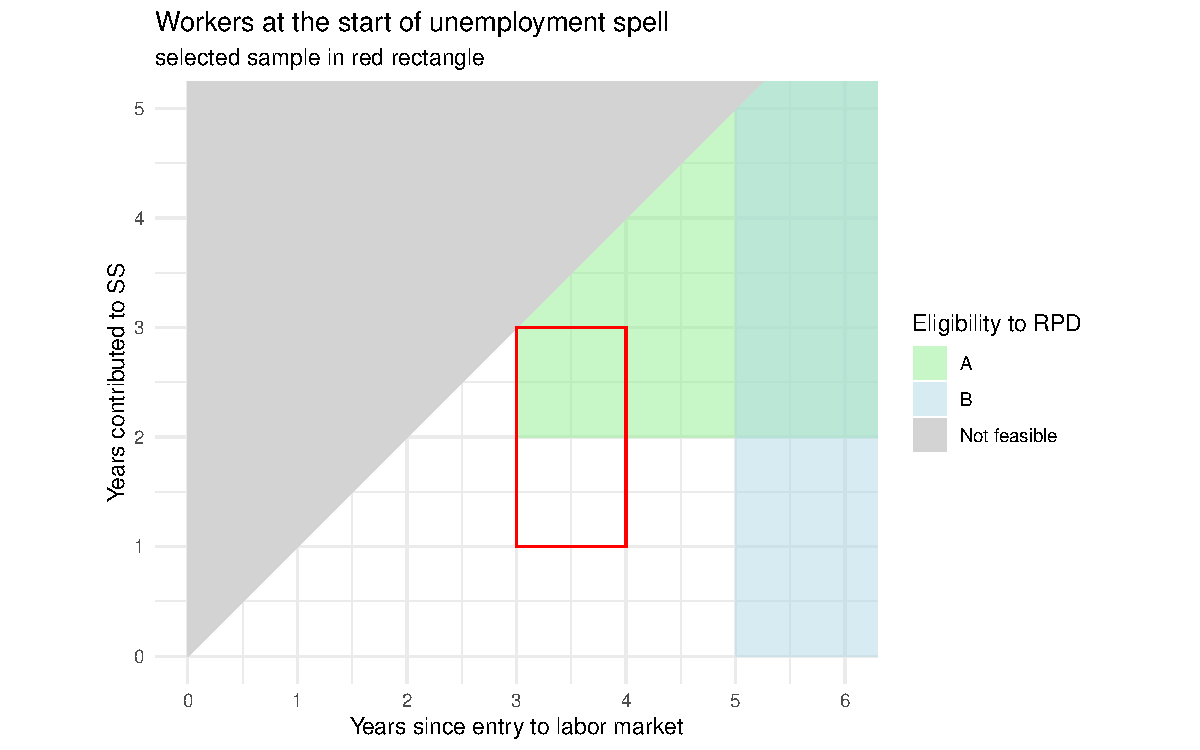
\includegraphics[keepaspectratio]{thesis_files/figure-pdf/unnamed-chunk-7-1.pdf}}

\emph{Note:} This figure shows (\emph{i}) sample means for evenly-spaced
14-day bins relative to the eligibility threshold, and (\emph{ii}) the
underlying regression function estimated using a triangular kernel,
optimal bandwidth and a linear local polynomial using Calonico,
Cattaneo, and Titiunik (\citeproc{ref-calonico2015}{2015}). The figure
shows workers' covariates do not systematically jump at the eligibility
threshold.

}

\end{figure}%

\begin{figure}

\caption{\label{fig-pre_unemp}Previous Job Outcomes around Eligibility
Threshold}

\centering{

\pandocbounded{\includegraphics[keepaspectratio]{thesis_files/figure-pdf/unnamed-chunk-8-1.pdf}}

\emph{Note:} his figure shows (\emph{i}) sample means for evenly-spaced
14-day bins relative to the eligibility threshold, and (\emph{ii}) the
underlying regression function estimated using a triangular kernel,
optimal bandwidth and a linear local polynomial using Calonico,
Cattaneo, and Titiunik (\citeproc{ref-calonico2015}{2015}). The figure
shows workers' previous job outcomes do not systematically jump at the
eligibility threshold.

}

\end{figure}%

\begin{table}

\caption{\label{tbl-covariates-bal}Eligibility Effect: Balance of
Covariates}

\centering{

\centering\centering
\resizebox{\ifdim\width>\linewidth\linewidth\else\width\fi}{!}{
\begin{tabular}[t]{>{\raggedright\arraybackslash}p{11em}>{\centering\arraybackslash}p{6em}>{\centering\arraybackslash}p{6em}>{\centering\arraybackslash}p{6em}>{\centering\arraybackslash}p{6em}>{\centering\arraybackslash}p{6em}}
\toprule
  & Female & Birth date & Began working & Unemployment date & Age\\
\midrule
RPD & \num{-0.001} & \num{-0.143} & \num{-0.005} & \num{-0.011} & \num{0.125}\\
 & (\num{0.005}) & (\num{0.059}) & (\num{0.022}) & (\num{0.022}) & (\num{0.051})\\
\midrule
Mean at cutoff - ineligible & 0.374 & 1,994 & 2,015 & 2,018 & 24.6\\
Observations & 877,749 & 847,714 & 877,749 & 877,749 & 847,714\\
\bottomrule
\end{tabular}}

\centering\centering
\resizebox{\ifdim\width>\linewidth\linewidth\else\width\fi}{!}{
\begin{threeparttable}
\begin{tabular}[t]{>{\raggedright\arraybackslash}p{11em}>{\centering\arraybackslash}p{6em}>{\centering\arraybackslash}p{6em}>{\centering\arraybackslash}p{6em}>{\centering\arraybackslash}p{6em}>{\centering\arraybackslash}p{6em}}
\toprule
  & Days since account opened & No CURP & Prev job duration (weeks) & Prev job total earnings & Prev job av monthly earnings\\
\midrule
RPD & \num{-2.124} & \num{-0.002} & \num{0.424} & \num{1634.627} & \num{311.151}\\
 & (\num{1.005}) & (\num{0.002}) & (\num{0.315}) & (\num{843.632}) & (\num{214.297})\\
\midrule
Mean at cutoff - ineligible & 1,268 & 0.0343 & 26.7 & 50,504 & 8,997\\
Observations & 877,749 & 877,749 & 877,749 & 877,749 & 877,749\\
\bottomrule
\end{tabular}
\begin{tablenotes}[para]
\item \textit{Note:} 
\item This table reports the estimated coefficient of interest from Equation 4.1, obtained using a local linear regression with a triangular kernel and optimal bandwidth selection. Bias-corrected point estimates and robust standard errors are computed following the procedure of Calonico, Cattaneo, and Titiunik (2014).
\end{tablenotes}
\end{threeparttable}}

}

\end{table}%

\chapter{Results}\label{sec-results}

This section presents the empirical results of the fuzzy regression
discontinuity design (RDD) used to estimate the causal effect of the
\emph{Retiro Parcial por Desempleo} (RPD) program on labor market
outcomes. I begin by documenting the first-stage effects of program
eligibility on take-up, which justifies the fuzzy RDD strategy. I then
estimate the local average treatment effect of RPD take-up on job search
behavior and medium-term labor market outcomes. The results are
complemented by a heterogeneity analysis that explores how these effects
vary by gender, income level, age, and exposure to the COVID-19
pandemic.

\section{First Stage}\label{sec-take-up}

This section presents evidence that workers eligible to the RPD program
(with at least two years of social security contributions at the time of
job displacement) are significantly more likely to take up than
ineligible workers. These first-stage results confirm three key points:
(i) the running variable has been correctly constructed, (ii) the first
stage of the fuzzy regression discontinuity design is strong, and (iii)
eligibility has a meaningful, albeit modest, effect on program take-up.

Figure~\ref{fig-first-stage} shows that displaced workers just above the
eligibility threshold are more likely to access the RPD program to
withdraw funds from their pension account. Inference from
Figure~\ref{fig-first-stage-path} and Table~\ref{tbl-take-up} confirms
that the take-up discontinuity is statistically significant and
stabilizes at around 4 percentage points after twelve months since
displacement.

Interestingly, Figure~\ref{fig-first-stage} shows that take-up increases
among initially ineligible workers after the twelfth month following
displacement. This pattern should not be interpreted as conventional
non-compliance. Rather, it reflects a change in eligibility status over
time. Under Eligibility Mode B, workers become eligible for the RPD
program once they accumulate at least five years of participation in the
formal labor market, regardless of their contribution history (see
Section~\ref{sec-context} and Figure~\ref{fig-eligibility}). Given that
the analytic sample is restricted to individuals displaced between their
third and fourth year in the formal sector, these workers only reach the
five-year threshold approximately one year after displacement. Once
eligible, they take up the program at rates comparable to the original
compliers, which accounts for the observed stabilization in the
intent-to-treat (ITT) effect after month 12 (see
Figure~\ref{fig-first-stage-path}).

Table~\ref{tbl-take-up} confirms that the ITT effect on program take-up
is highly statistically significant, albeit small in magnitude. This
justifies the use of a fuzzy RDD strategy to estimate the local average
treatment effect of RPD on labor market outcomes among compliers. The
modest size of the first-stage effect is consistent with the
institutional design of the RPD program: unlike traditional unemployment
insurance schemes, RPD allows only a partial withdrawal from workers'
own pension accounts. It is, by design, a self-financed benefit that
internalizes the cost of unemployment support.

\begin{figure}

\caption{\label{fig-first-stage}Eligibility Effect on Take Up}

\centering{

\pandocbounded{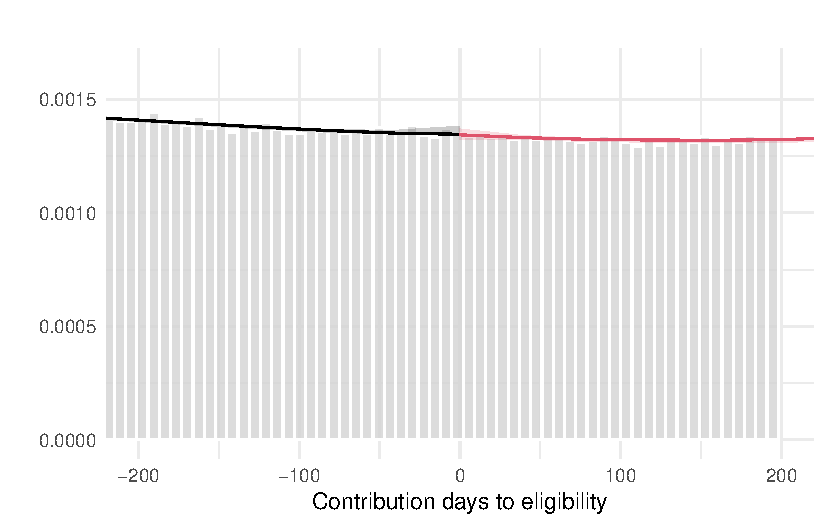
\includegraphics[keepaspectratio]{thesis_files/figure-pdf/unnamed-chunk-9-1.pdf}}

Note: This figure displays (i) sample means calculated within evenly
spaced 14-day bins relative to the eligibility threshold, and (ii) the
estimated regression function obtained using a local linear polynomial
with a triangular kernel and optimal bandwidth selection following the
method of Calonico, Cattaneo, and Titiunik
(\citeproc{ref-calonico2015}{2015}). The results show a discrete
increase in program take-up at the eligibility threshold.

}

\end{figure}%

\begin{figure}

\caption{\label{fig-first-stage-path}Dynamic Effect of Eligibility on
Take Up}

\centering{

\pandocbounded{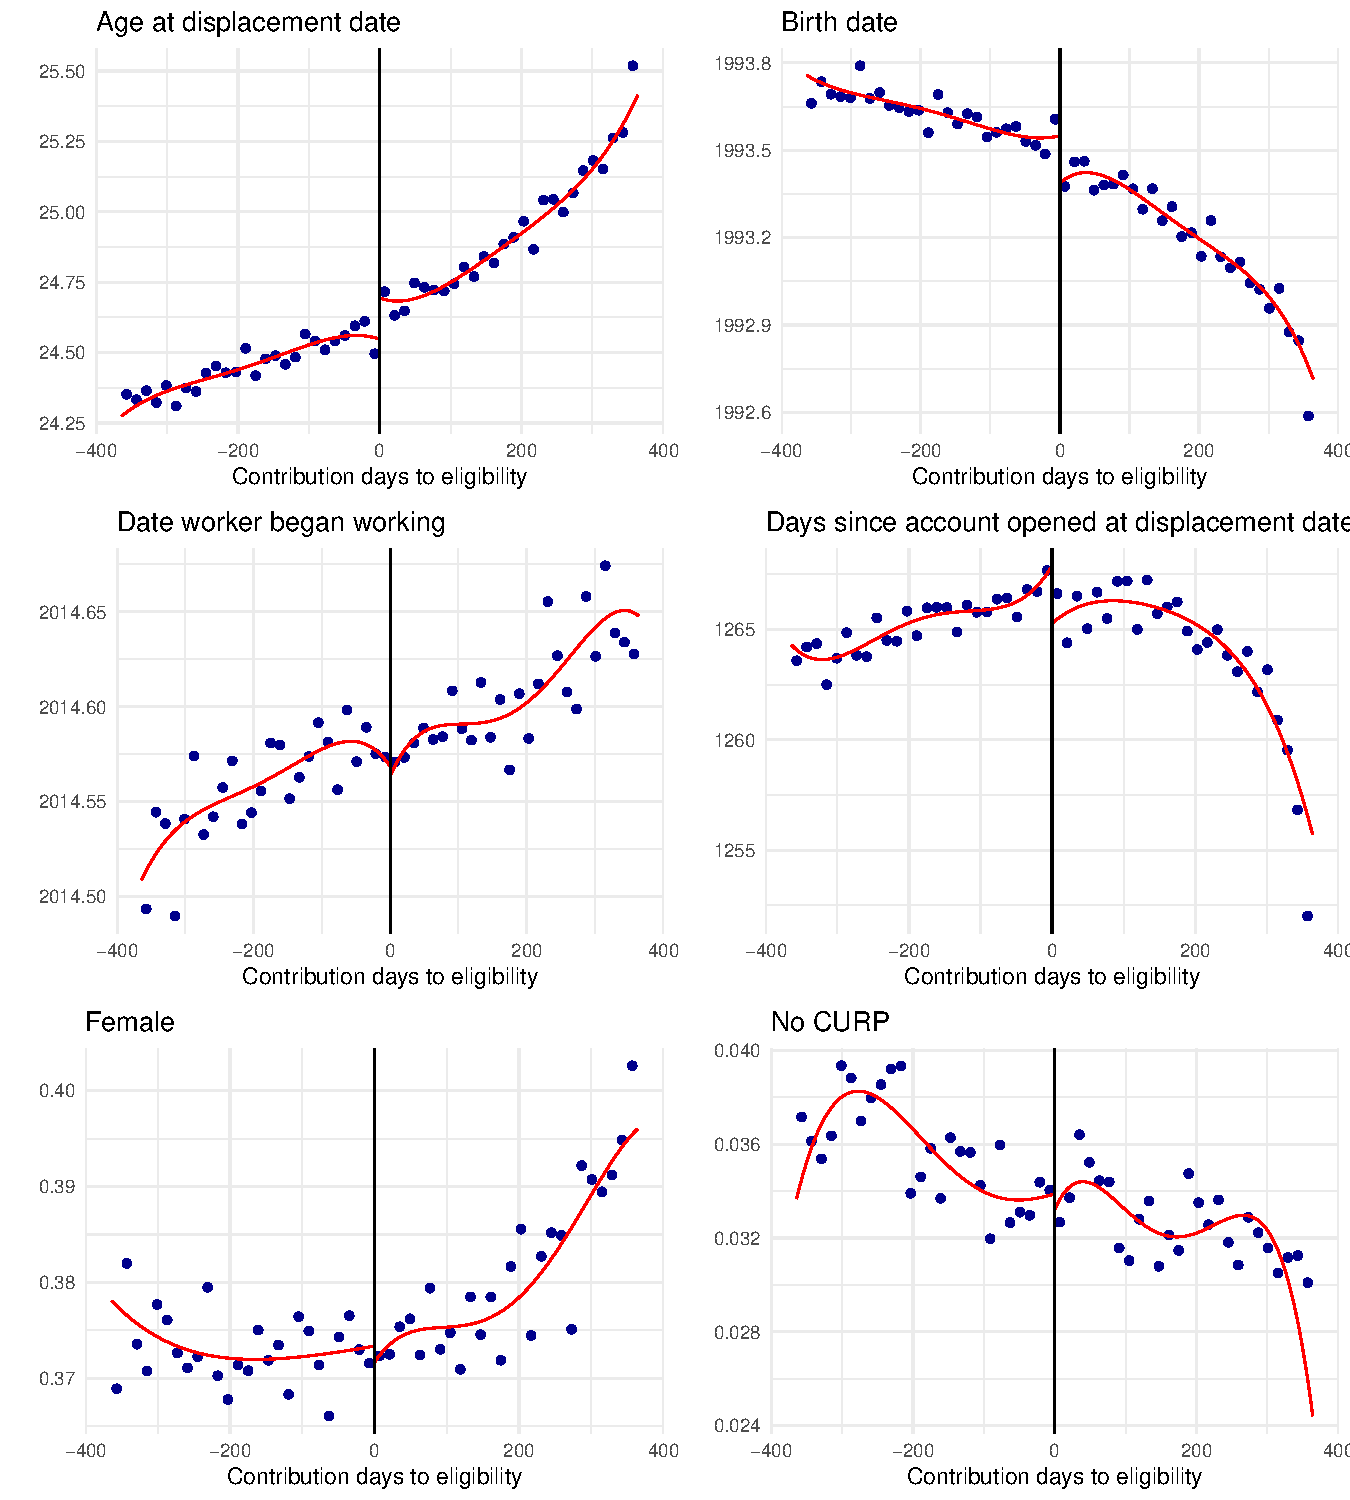
\includegraphics[keepaspectratio]{thesis_files/figure-pdf/unnamed-chunk-10-1.pdf}}

Note: This figure presents the estimated coefficients of interest from
Equation~\ref{eq-1s}. Estimates are obtained using a local linear
regression with a triangular kernel and optimal bandwidth selection.
Bias-corrected point estimates and robust standard errors are computed
following the method of Calonico, Cattaneo, and Titiunik
(\citeproc{ref-calonico2014}{2014}). Vertical lines across point
estimates represent 95\% confidence intervals.

}

\end{figure}%

\begin{table}

\caption{\label{tbl-take-up}Eligibility Effect: First Stage}

\centering{

\centering\centering
\resizebox{\ifdim\width>\linewidth\linewidth\else\width\fi}{!}{
\begin{threeparttable}
\begin{tabular}[t]{>{\raggedright\arraybackslash}p{11em}>{\centering\arraybackslash}p{5em}>{\centering\arraybackslash}p{5em}>{\centering\arraybackslash}p{5em}>{\centering\arraybackslash}p{5em}>{\centering\arraybackslash}p{5em}}
\toprule
  & Take up - 2 months & Take up - 3 months & Take up - 6 months & Take up - 9 months & Take up - 12 months\\
\midrule
RPD & \num{0.008} & \num{0.014} & \num{0.027} & \num{0.033} & \num{0.036}\\
 & (\num{0.001}) & (\num{0.002}) & (\num{0.002}) & (\num{0.003}) & (\num{0.003})\\
\midrule
Mean at cutoff - ineligible & 0.00174 & 0.00602 & 0.0133 & 0.0187 & 0.0231\\
Observations & 877,749 & 877,749 & 877,749 & 877,749 & 877,749\\
\bottomrule
\end{tabular}
\begin{tablenotes}[para]
\item \textit{Note:} 
\item This table reports the estimated coefficient of interest from Equation 4.1, obtained using a local linear regression with a triangular kernel and optimal bandwidth selection. Bias-corrected point estimates and robust standard errors are computed following the procedure of Calonico, Cattaneo, and Titiunik (2014).
\end{tablenotes}
\end{threeparttable}}

}

\end{table}%

\section{Job Search Outcomes}\label{sec-main-results}

I now turn to the effects of RPD take-up on labor market outcomes,
estimated using the fuzzy regression discontinuity design described in
Equation~\ref{eq-2s}. Figure~\ref{fig-fuzzy-path} and
Table~\ref{tbl-fuzzy-job-search-1} present the dynamic treatment effects
on unemployment duration and employment survival. By three months after
displacement, taking up RPD increases the probability of remaining
unemployed (i.e., survival in unemployment) by 31 percentage points.
After 36 months, the cumulative effect on unemployment duration amounts
to 36 additional weeks. These effects are statistically significant at
the 5\% level and align with the broader empirical literature: income
support during unemployment typically prolongs joblessness. At the
eligibility cutoff, RPD users experience a 70\% increase in unemployment
duration relative to non-eligible workers after three years. These
findings underscore the potential social costs of income-substitution
programs such as RPD, particularly through the lens of forgone
contributions to the social security system due to extended
non-employment spells.

For completeness, Appendix Figure~\ref{fig-survival},
Figure~\ref{fig-duration}, and Figure~\ref{fig-path}, along with
Table~\ref{tbl-job-search}, present intention-to-treat (ITT) estimates
for the same outcomes, as described in Equation~\ref{eq-1s}, as well as
the corresponding RD plots. The ITT estimates show smaller effects than
those reported in comparable international settings. For instance,
Britto (\citeproc{ref-britto2022}{2022}) finds that a lump-sum
unemployment benefit program in Brazil increased employment survival by
1.9 percentage points after three months, whereas the estimated effect
of RPD is just 0.7 percentage points over the same period. Similarly,
Velázquez Guadarrama (\citeproc{ref-veluxe1zquezguadarrama2023}{2023}),
using ENOE survey data, reports that eligibility to RPD increases
unemployment duration by 11.8 weeks (or 82.85 days), while the ITT
estimate from this study points to a much smaller increase of just 0.65
weeks over a three-year horizon. Importantly, none of the ITT estimates
reported here are statistically significant at the 5\% level.

Turning to employment quality, Table Table~\ref{tbl-fuzzy-job-search-2}
reports the estimated effects of RPD take-up on post-displacement
outcomes such as earnings and job duration. The composition of
re-employed workers appears similar around the eligibility threshold in
terms of prior earnings (see column 4), suggesting no substantial
selection effects. However, there is limited evidence that RPD take-up
improves subsequent job quality. While the point estimate for monthly
earnings in the next job suggests a sizeable increase---more than a
100\% gain relative to pre-displacement wages, or approximately \$9,500
MXN---this estimate is only significant at the 10\% level. Moreover, the
effects on next job cumulative earnings and job duration are
statistically indistinguishable from zero.

When placed in context with the existing literature, these ITT results
point to a mixed picture. (\citeproc{ref-britto}{\textbf{britto?}})
finds a statistically significant 1.7\% decline in annual earnings
associated with Brazil's program, while eligibility for RPD is
associated with a non-significant 4.6\% increase. Velázquez Guadarrama
(\citeproc{ref-veluxe1zquezguadarrama2023}{2023}), using ENOE data,
finds a smaller yet statistically significant increase of 2.47\% in wage
income among eligible workers. Overall, while some point estimates
suggest potentially positive effects of RPD on earnings, the lack of
statistical significance and the inconsistency with prior studies call
for cautious interpretation.

\begin{figure}

\caption{\label{fig-fuzzy-path}Dynamic Effect of RPD on Survival and
Duration of Unemployment}

\centering{

\pandocbounded{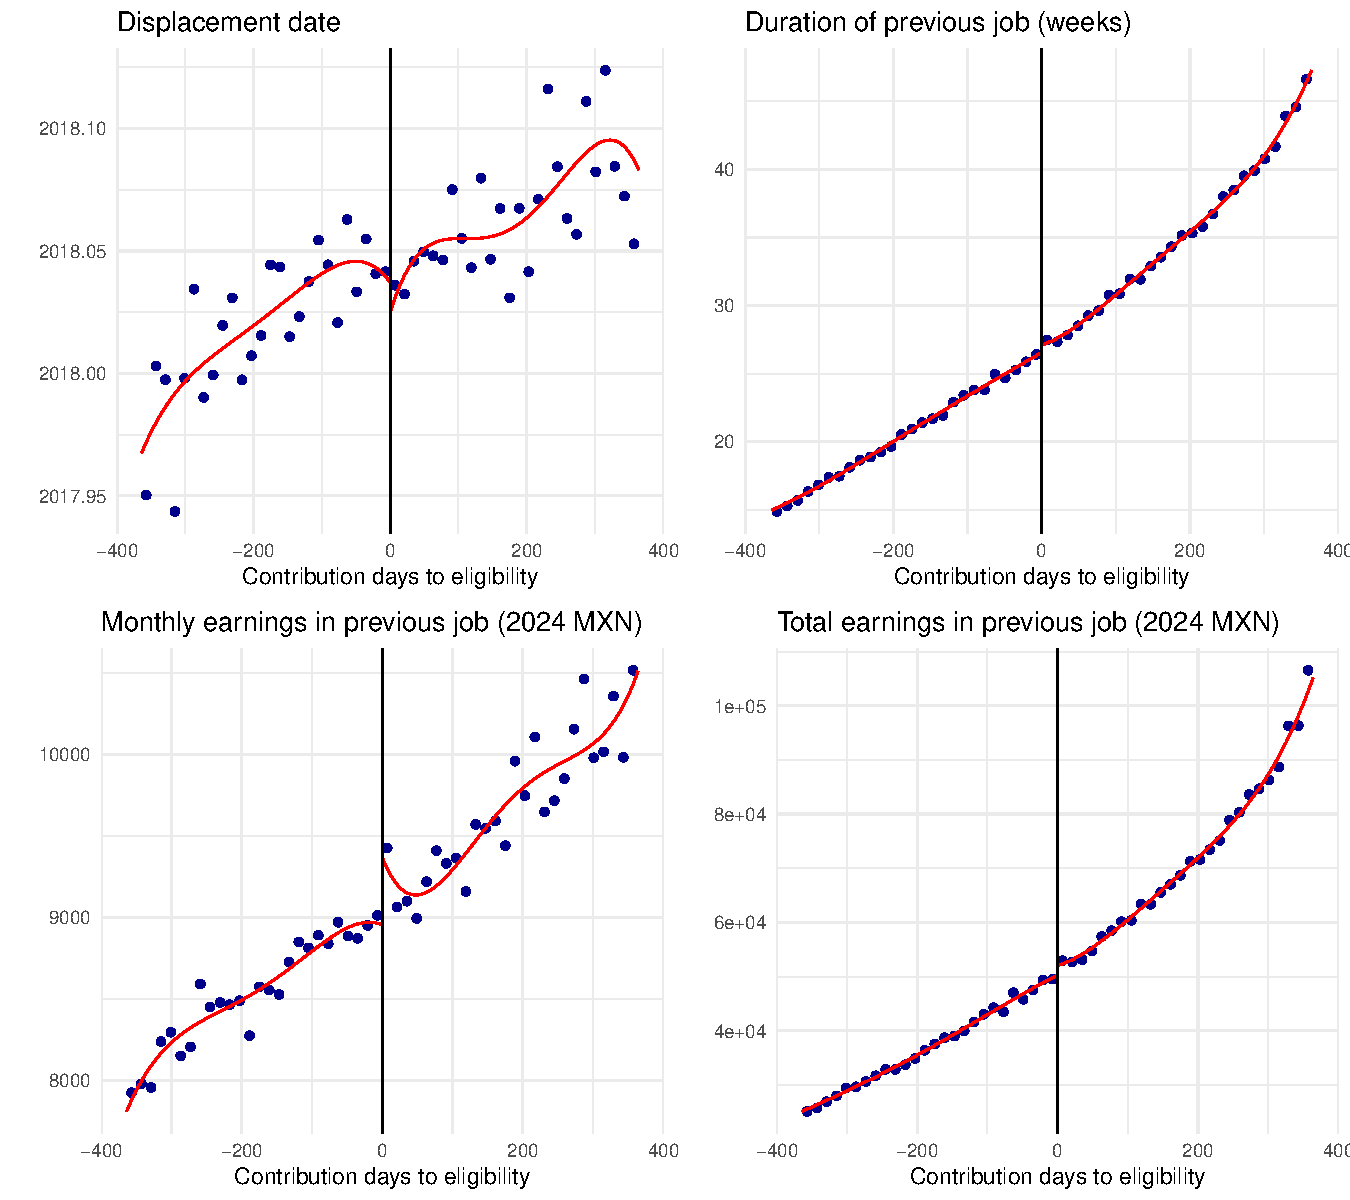
\includegraphics[keepaspectratio]{thesis_files/figure-pdf/unnamed-chunk-11-1.pdf}}

Note: This figure presents the estimated coefficients of interest from
Equation~\ref{eq-2s}. Estimates are obtained using a local linear
regression with a triangular kernel and optimal bandwidth selection.
Bias-corrected point estimates and robust standard errors are computed
following the method of Calonico, Cattaneo, and Titiunik
(\citeproc{ref-calonico2014}{2014}). Vertical lines across point
estimates represent 95\% confidence intervals.

}

\end{figure}%

\begin{table}

\caption{\label{tbl-fuzzy-job-search}RPD Effect: Job Search Outcomes}

\begin{minipage}{\linewidth}

\subcaption{\label{tbl-fuzzy-job-search-1}Survival and Duration of
Unemployment}

\centering{

\centering\centering
\resizebox{\ifdim\width>\linewidth\linewidth\else\width\fi}{!}{
\fontsize{8}{10}\selectfont
\begin{tabular}[t]{>{\raggedright\arraybackslash}p{11em}>{\centering\arraybackslash}p{6em}>{\centering\arraybackslash}p{6em}>{\centering\arraybackslash}p{6em}>{\centering\arraybackslash}p{6em}}
\toprule
  & Survival - 3 months & Survival - 36 months & Duration - 6 months (wks) & Duration - 36 months (wks)\\
\midrule
RPD & \num{0.31} & \num{0.06} & \num{4.85} & \num{36.27}\\
 & (\num{0.15}) & (\num{0.07}) & (\num{2.37}) & (\num{15.86})\\
\midrule
Mean at cutoff - ineligible & 0.778 & 0.106 & 20.5 & 51.5\\
Observations & 877,749 & 877,749 & 877,749 & 877,749\\
\bottomrule
\end{tabular}}

}

\end{minipage}%
\newline
\begin{minipage}{\linewidth}

\subcaption{\label{tbl-fuzzy-job-search-2}Next Job Quality}

\centering{

\centering\centering
\resizebox{\ifdim\width>\linewidth\linewidth\else\width\fi}{!}{
\fontsize{8}{10}\selectfont
\begin{threeparttable}
\begin{tabular}[t]{>{\raggedright\arraybackslash}p{11em}>{\centering\arraybackslash}p{6em}>{\centering\arraybackslash}p{6em}>{\centering\arraybackslash}p{6em}>{\centering\arraybackslash}p{6em}}
\toprule
  & Monthly earnings & Total earnings & Job duration (weeks) & Prev. job earnings\\
\midrule
RPD & \num{9428.61} & \num{67095.54} & \num{16.49} & \num{9626.59}\\
 & (\num{4882.68}) & (\num{61137.52}) & (\num{14.54}) & (\num{6055.86})\\
\midrule
Mean at cutoff - ineligible & 8,327 & 87,306 & 35.7 & 9,005\\
Observations & 873,434 & 873,434 & 873,434 & 873,434\\
\bottomrule
\end{tabular}
\begin{tablenotes}[para]
\item \textit{Note:} 
\item This table reports the estimated coefficient of interest from Equation 4.2, where treatment is defined as program take-up 12 months after displacement. Estimates are obtained using a local linear regression with a triangular kernel and optimal bandwidth selection. Bias-corrected point estimates and robust standard errors are computed following the method of Cattaneo, Idrobo, and Titiunik (2024). Currencies are expressed in 2024 Mexican Pesos.
\end{tablenotes}
\end{threeparttable}}

}

\end{minipage}%

\end{table}%

\section{Medium Term Effects}\label{sec-medium-run}

This section examines the medium-term labor market outcomes associated
with participation in the RPD program. Table~\ref{tbl-medium-fuzzy}
reports the estimated effects for RPD users, computed using the fuzzy
regression discontinuity design described in Equation~\ref{eq-2s}.
Although none of the estimates reach statistical significance at the 5\%
level, the results suggest a persistent decline in formal labor earnings
over the three-year post-displacement period. This decline appears to be
driven entirely by the extensive margin, as RPD recipients were employed
for fewer months and, on average, reported no wage earnings.

While most effects are not statistically distinguishable from zero, they
may reflect longer-lasting disruptions in formal labor market
attachment. Taken together, these findings indicate that the RPD program
not only extends the duration of unemployment but also fails to enhance
post-displacement job quality or promote higher long-term earnings in
the formal sector---contrary to the predictions of the more optimistic
unemployment insurance literature (\citeproc{ref-acemoglu1999}{Acemoglu
and Shimer 1999}, \citeproc{ref-acemoglu2000}{2000}).

\begin{table}

\caption{\label{tbl-medium-fuzzy}RPD Effect: Earnings, Employment and
Wages over Medium Term}

\begin{minipage}{\linewidth}

\subcaption{\label{tbl-medium-fuzzy-1}Earnings}

\centering{

\centering\centering
\resizebox{\ifdim\width>\linewidth\linewidth\else\width\fi}{!}{
\begin{tabular}[t]{>{\raggedright\arraybackslash}p{11em}>{\centering\arraybackslash}p{6em}>{\centering\arraybackslash}p{6em}>{\centering\arraybackslash}p{6em}>{\centering\arraybackslash}p{6em}}
\toprule
  & Total 3 years & Year 1 & Year 2 & Year 3\\
\midrule
RPD & \num{-20378.63} & \num{-13116.15} & \num{-16418.20} & \num{-3121.18}\\
 & (\num{44061.00}) & (\num{12983.56}) & (\num{17775.58}) & (\num{24304.58})\\
\midrule
Mean at cutoff - ineligible & 148,762 & 31,965 & 54,471 & 62,345\\
Observations & 877,749 & 877,749 & 877,749 & 877,749\\
\bottomrule
\end{tabular}}

}

\end{minipage}%
\newline
\begin{minipage}{\linewidth}

\subcaption{\label{tbl-medium-fuzzy-2}Months Worked}

\centering{

\centering\centering
\resizebox{\ifdim\width>\linewidth\linewidth\else\width\fi}{!}{
\begin{tabular}[t]{>{\raggedright\arraybackslash}p{11em}>{\centering\arraybackslash}p{6em}>{\centering\arraybackslash}p{6em}>{\centering\arraybackslash}p{6em}>{\centering\arraybackslash}p{6em}}
\toprule
  & Total 3 years & Year 1 & Year 2 & Year 3\\
\midrule
RPD & \num{-1.41} & \num{-1.95} & \num{-0.57} & \num{-0.15}\\
 & (\num{2.65}) & (\num{1.26}) & (\num{1.12}) & (\num{1.42})\\
\midrule
Mean at cutoff - ineligible & 15.3 & 3.8 & 5.67 & 5.86\\
Observations & 877,749 & 877,749 & 877,749 & 877,749\\
\bottomrule
\end{tabular}}

}

\end{minipage}%
\newline
\begin{minipage}{\linewidth}

\subcaption{\label{tbl-medium-fuzzy-3}Average Monthly Earnings}

\centering{

\centering\centering
\resizebox{\ifdim\width>\linewidth\linewidth\else\width\fi}{!}{
\begin{threeparttable}
\begin{tabular}[t]{>{\raggedright\arraybackslash}p{11em}>{\centering\arraybackslash}p{6em}>{\centering\arraybackslash}p{6em}>{\centering\arraybackslash}p{6em}>{\centering\arraybackslash}p{6em}}
\toprule
  & Total 3 years & Year 1 & Year 2 & Year 3\\
\midrule
RPD & \num{903.31} & \num{634.12} & \num{-1806.90} & \num{-259.16}\\
 & (\num{1808.21}) & (\num{1814.44}) & (\num{1954.97}) & (\num{2146.99})\\
\midrule
Mean at cutoff - ineligible & 8,903 & 8,012 & 8,959 & 9,902\\
Observations & 794,688 & 578,415 & 650,874 & 633,586\\
\bottomrule
\end{tabular}
\begin{tablenotes}[para]
\item \textit{Note:} 
\item This table reports the estimated coefficient of interest from Equation 4.2, where treatment is defined as program take-up 12 months after displacement. Estimates are obtained using a local linear regression with a triangular kernel and optimal bandwidth selection. Bias-corrected point estimates and robust standard errors are computed following the method of Cattaneo, Idrobo, and Titiunik (2024). Currencies are expressed in 2024 Mexican Pesos.
\end{tablenotes}
\end{threeparttable}}

}

\end{minipage}%

\end{table}%

\section{Additional Results: Heterogeneous Treatment
Effects}\label{sec-additional-results}

In this section, I present additional results on the heterogeneity of
the effect of the RPD program on labor market outcomes. I explore the
heterogeneity of the treatment effect by age, wage, and exposure to
COVID-19 in Table~\ref{tbl-income}, Table~\ref{tbl-age}, and
Table~\ref{tbl-covid}, respectively.

\textbf{Income.} Table~\ref{tbl-income} explores heterogeneous effects
of the RPD program by pre-displacement income, dividing the sample at
the median wage in the previous job (\$6,669.2 MXN). Take-up rates do
not differ significantly between the above- and below-median wage
groups, suggesting comparable levels of program engagement across income
levels.

However, the impact on labor market outcomes varies substantially. Among
workers earning below the median, the RPD significantly increases the
probability of remaining unemployed within the first three months
following displacement. Over a 36-month horizon, the effect on
unemployment duration for this group is nearly ten times larger than for
their higher-income counterparts, indicating a much more pronounced and
persistent detachment from formal employment among lower-wage workers.

In terms of reemployment outcomes, RPD recipients with above-median
pre-displacement wages secure jobs that pay approximately 67\% more than
those obtained by ineligible workers. In contrast, no statistically
significant effect is found on the wages of reemployed workers in the
below-median group. Over the full three-year horizon, higher-income
workers exhibit a positive, albeit imprecise, impact on total earnings.
Meanwhile, lower-income workers experience an average earnings loss of
approximately \$40,000 MXN---driven by prolonged unemployment and the
absence of wage gains upon reemployment---although this estimate is not
statistically distinguishable from zero.

These findings highlight the importance of accounting for income
heterogeneity in program design. In the case of the RPD, the structure
of benefits may inadvertently reinforce existing inequalities---offering
greater long-term advantages to relatively better-off workers, while
leaving lower-wage workers worse off in both employment duration and
earnings trajectories.

\textbf{Age.} Table~\ref{tbl-age} examines heterogeneous effects of the
RPD program by age at the time of displacement, dividing the sample at
the median age of 22.9 years. As with income, take-up rates do not
differ significantly between younger and older workers, indicating
comparable engagement with the program across age groups.

The effects on unemployment duration are not statistically significant
for either group over the short (3-month) or medium (36-month) horizons.
However, point estimates suggest meaningful differences in magnitude. By
three months, younger workers exhibit a 23 percentage point increase in
the probability of remaining unemployed, compared to only a 10
percentage point increase for older workers---more than twice the
effect. This disparity widens substantially over time: after 36 months,
the cumulative increase in unemployment duration is 35 weeks for younger
workers, compared to just 3 weeks for older workers---an effect nearly
ten times larger.

In contrast, there is no clear evidence of differential effects on
post-displacement job quality. All estimates related to wages and job
duration in the next job are statistically indistinguishable from zero
for both age groups.

Over the full three-year horizon, younger workers appear to experience
greater earnings losses. On average, they earned approximately \$20,000
MXN less than their counterparts who were not eligible for RPD, compared
to a \$9,000 MXN loss among older workers. These estimates, however, are
imprecise and should be interpreted with caution.

Taken together, these findings suggest that age is an important
dimension of heterogeneity in the effects of unemployment assistance
programs. In the case of the RPD, younger workers may face more
persistent labor market disruptions, with weaker labor market
attachement, potentially compounding early-career vulnerabilities.

\textbf{Gender.} Table~\ref{tbl-gender} examines the heterogeneous
effects of the RPD program by gender. Panel A presents results for
males, while Panel B reports estimates for females. Take-up rates are
similar across groups, with no statistically significant gender
differences in program participation 12 months after displacement.

However, the effects on labor market outcomes diverge markedly by
gender. Among males, RPD take-up increases the probability of remaining
unemployed three months after displacement by 40 percentage points. This
effect persists over time, resulting in a cumulative increase in
unemployment duration of 49 weeks over the subsequent three years---an
effect that is both large and statistically significant. In contrast,
female recipients exhibit no significant change in short-term survival
or long-term unemployment duration. The point estimate for unemployment
duration is actually negative (--8.7 weeks), but imprecisely estimated.

Differences in earnings outcomes are similarly pronounced. Male RPD
recipients experience large, positive effects on monthly earnings in
their next job---approximately \$11,252 MXN higher than ineligible
males---and a cumulative three-year earnings gain of \$1,066 MXN. These
estimates, while imprecise, suggest a potential improvement in job
quality among men. In contrast, female RPD recipients see no significant
gain in monthly earnings and suffer an average three-year total earnings
loss of \$16,126 MXN. This reduction in earnings is likely driven by
delayed labor market reentry and the absence of wage gains upon
reemployment.

Interestingly, the margin of adjustment differs across genders. Male
recipients work 2.7 fewer months over the three-year period, while
female recipients actually work 1.5 months more. Yet, the increase in
work months among women does not translate into earnings gains, possibly
reflecting reemployment in lower-wage or more precarious jobs.

Taken together, these findings highlight significant gender disparities
in the labor market effects of the RPD program. While male recipients
face longer unemployment durations, they appear to recover through
access to better-paying jobs. Female recipients, in contrast, do not
experience improvements in job quality and incur significant earnings
losses. These results underscore the need for gender-sensitive design in
unemployment support policies, as uniform benefit structures may yield
unequal labor market outcomes.

\textbf{Exposure to COVID-19.} Table~\ref{tbl-covid} explores
heterogeneous effects of the RPD program based on whether individuals
were displaced before or after the onset of the COVID-19 pandemic. Panel
A includes workers who were displaced before March 2019, and thus had at
least a full year of unemployment before the pandemic hit in March 2020.
These individuals are considered to have no exposure to pandemic-related
labor market disruptions during their initial post-displacement period.
Panel B, by contrast, focuses on individuals displaced after March 2020,
who faced full exposure to the labor market conditions created by the
pandemic.

First-stage estimates show that take-up rates are slightly lower among
post-pandemic displacees (3\%) than among pre-pandemic ones (4\%),
although the difference is modest. However, labor market outcomes
diverge sharply across cohorts.

Among workers with no exposure to the pandemic (Panel A), RPD take-up
leads to substantial and significant increases in unemployment duration.
The probability of remaining unemployed at 3 months rises by 37
percentage points, and cumulative unemployment duration increases by
over 52 weeks---essentially one additional year of joblessness. Despite
these adverse effects on employment continuity, there is a modest
increase in monthly earnings in the next job (12,416 MXN), although
total earnings over the three-year horizon fall by 8,539 MXN, suggesting
that the gains in job quality do not fully offset the costs of prolonged
unemployment.

In contrast, among workers fully exposed to the COVID-19 crisis (Panel
B), RPD take-up is associated with much weaker effects on labor market
behavior. The effect on 3-month survival is negligible (1 pp), and the
cumulative increase in unemployment duration is only 22 weeks.
Strikingly, reemployment outcomes for this group appear worse: RPD
recipients experience a decline in job duration (--9.4 weeks) and a
relatively small increase in next-job earnings (5,011 MXN). However,
despite weaker job quality indicators, total earnings over the
three-year period rise by 37,277 MXN---likely due to higher reemployment
rates and a labor market rebound post-pandemic.

These results suggest that the macroeconomic context at the time of
displacement plays a crucial role in shaping the effects of unemployment
assistance. While RPD recipients displaced before COVID-19 faced steep
penalties in terms of extended non-employment and modest earnings gains,
those displaced during the pandemic experienced smaller disruptions and
more favorable cumulative earnings trajectories. Importantly, this
contrast highlights the interaction between individual-level support
programs and broader labor market conditions: a well-timed benefit may
facilitate recovery in a tightening labor market, while the same benefit
in a more stable environment may prolong detachment without improving
long-term outcomes.

\begin{table}

\caption{\label{tbl-income}RPD Effect: Heterogeneity over Wage}

\begin{minipage}{\linewidth}

\subcaption{\label{tbl-income-1}Below Median Wage}

\centering{

\centering\centering
\resizebox{\ifdim\width>\linewidth\linewidth\else\width\fi}{!}{
\fontsize{8}{10}\selectfont
\begin{tabular}[t]{>{\raggedright\arraybackslash}p{12em}>{\centering\arraybackslash}p{4.5em}>{\centering\arraybackslash}p{4.5em}>{\centering\arraybackslash}p{4.5em}>{\centering\arraybackslash}p{4.5em}>{\centering\arraybackslash}p{4.5em}>{\centering\arraybackslash}p{4.5em}>{\centering\arraybackslash}p{4.5em}>{\centering\arraybackslash}p{4.5em}}
\toprule
  & Take up (First stage) & Survival - 3 months & Duration - 36 months (wks) & Job duration (wks) & Monthly Earnings & Total Earnings - 3 years & Months Worked - 3 years & Monthly Earnings - 3 years\\
\midrule
RPD & \num{0.04} & \num{0.38} & \num{46.16} & \num{15.80} & \num{4737.20} & \num{-39836.31} & \num{-3.64} & \num{-60.70}\\
 & (\num{0.00}) & (\num{0.14}) & (\num{17.22}) & (\num{21.26}) & (\num{5196.56}) & (\num{38497.50}) & (\num{3.41}) & (\num{1467.20})\\
\midrule
Mean at cutoff - ineligible & 0.0121 & 0.797 & 53.8 & 36.2 & 7,269 & 119,239 & 14.6 & 7,617\\
Observations & 438,875 & 438,875 & 438,875 & 436,925 & 436,925 & 438,875 & 438,875 & 393,137\\
\bottomrule
\end{tabular}}

}

\end{minipage}%
\newline
\begin{minipage}{\linewidth}

\subcaption{\label{tbl-income-2}Above Median Wage}

\centering{

\centering\centering
\resizebox{\ifdim\width>\linewidth\linewidth\else\width\fi}{!}{
\fontsize{8}{10}\selectfont
\begin{threeparttable}
\begin{tabular}[t]{>{\raggedright\arraybackslash}p{12em}>{\centering\arraybackslash}p{4.5em}>{\centering\arraybackslash}p{4.5em}>{\centering\arraybackslash}p{4.5em}>{\centering\arraybackslash}p{4.5em}>{\centering\arraybackslash}p{4.5em}>{\centering\arraybackslash}p{4.5em}>{\centering\arraybackslash}p{4.5em}>{\centering\arraybackslash}p{4.5em}}
\toprule
  & Take up (First stage) & Survival - 3 months & Duration - 36 months (wks) & Job duration (wks) & Monthly Earnings & Total Earnings - 3 years & Months Worked - 3 years & Monthly Earnings - 3 years\\
\midrule
RPD & \num{0.04} & \num{-0.05} & \num{-4.67} & \num{17.05} & \num{6416.72} & \num{17516.18} & \num{0.66} & \num{2081.56}\\
 & (\num{0.00}) & (\num{0.14}) & (\num{15.71}) & (\num{21.47}) & (\num{3044.42}) & (\num{73028.49}) & (\num{4.21}) & (\num{2808.53})\\
\midrule
Mean at cutoff - ineligible & 0.027 & 0.763 & 49.7 & 35.2 & 9,437 & 178,004 & 16 & 10,180\\
Observations & 438,874 & 438,874 & 438,874 & 436,509 & 436,509 & 438,874 & 438,874 & 401,551\\
\bottomrule
\end{tabular}
\begin{tablenotes}[para]
\item \textit{Note:} 
\item This table reports the estimated coefficient of interest from Equation 4.1, obtained using a local linear regression with a triangular kernel and optimal bandwidth selection. Bias-corrected point estimates and robust standard errors are computed following the procedure of Calonico, Cattaneo, and Titiunik (2014). Panel A reports results for individuals whose earnings in their previous job were below the sample median wage (\$6,669.2), while Panel B reports results for those above the median. All monetary values are expressed in 2024 Mexican Pesos.
\end{tablenotes}
\end{threeparttable}}

}

\end{minipage}%

\end{table}%

\begin{table}

\caption{\label{tbl-age}RPD Effect: Heterogeneity over Age}

\begin{minipage}{\linewidth}

\subcaption{\label{tbl-age-1}Below Median Age}

\centering{

\centering\centering
\resizebox{\ifdim\width>\linewidth\linewidth\else\width\fi}{!}{
\fontsize{8}{10}\selectfont
\begin{tabular}[t]{>{\raggedright\arraybackslash}p{12em}>{\centering\arraybackslash}p{4.5em}>{\centering\arraybackslash}p{4.5em}>{\centering\arraybackslash}p{4.5em}>{\centering\arraybackslash}p{4.5em}>{\centering\arraybackslash}p{4.5em}>{\centering\arraybackslash}p{4.5em}>{\centering\arraybackslash}p{4.5em}>{\centering\arraybackslash}p{4.5em}}
\toprule
  & Take up (First stage) & Survival - 3 months & Duration - 36 months (wks) & Job duration (wks) & Monthly Earnings & Total Earnings - 3 years & Months Worked - 3 years & Monthly Earnings - 3 years\\
\midrule
RPD & \num{0.04} & \num{0.23} & \num{35.16} & \num{-4.43} & \num{60.02} & \num{-20965.39} & \num{-2.11} & \num{357.61}\\
 & (\num{0.00}) & (\num{0.17}) & (\num{17.98}) & (\num{18.77}) & (\num{1805.32}) & (\num{42939.90}) & (\num{3.82}) & (\num{1261.62})\\
\midrule
Mean at cutoff - ineligible & 0.0162 & 0.767 & 47.7 & 33.4 & 7,747 & 141,633 & 15.9 & 8,327\\
Observations & 423,857 & 423,857 & 423,857 & 422,155 & 422,155 & 423,857 & 423,857 & 388,767\\
\bottomrule
\end{tabular}}

}

\end{minipage}%
\newline
\begin{minipage}{\linewidth}

\subcaption{\label{tbl-age-2}Above Median Age}

\centering{

\centering\centering
\resizebox{\ifdim\width>\linewidth\linewidth\else\width\fi}{!}{
\fontsize{8}{10}\selectfont
\begin{threeparttable}
\begin{tabular}[t]{>{\raggedright\arraybackslash}p{12em}>{\centering\arraybackslash}p{4.5em}>{\centering\arraybackslash}p{4.5em}>{\centering\arraybackslash}p{4.5em}>{\centering\arraybackslash}p{4.5em}>{\centering\arraybackslash}p{4.5em}>{\centering\arraybackslash}p{4.5em}>{\centering\arraybackslash}p{4.5em}>{\centering\arraybackslash}p{4.5em}}
\toprule
  & Take up (First stage) & Survival - 3 months & Duration - 36 months (wks) & Job duration (wks) & Monthly Earnings & Total Earnings - 3 years & Months Worked - 3 years & Monthly Earnings - 3 years\\
\midrule
RPD & \num{0.04} & \num{0.10} & \num{3.10} & \num{28.18} & \num{9759.34} & \num{-9224.03} & \num{-1.35} & \num{114.08}\\
 & (\num{0.00}) & (\num{0.12}) & (\num{16.58}) & (\num{19.68}) & (\num{6752.33}) & (\num{59252.06}) & (\num{3.75}) & (\num{2246.94})\\
\midrule
Mean at cutoff - ineligible & 0.0214 & 0.793 & 56.1 & 38.4 & 9,032 & 157,792 & 14.9 & 9,601\\
Observations & 423,857 & 423,857 & 423,857 & 421,318 & 421,318 & 423,857 & 423,857 & 378,703\\
\bottomrule
\end{tabular}
\begin{tablenotes}[para]
\item \textit{Note:} 
\item This table reports the estimated coefficient of interest from Equation 4.2, where treatment is defined as program take-up 12 months after displacement. Estimates are obtained using a local linear regression with a triangular kernel and optimal bandwidth selection. Bias-corrected point estimates and robust standard errors are computed following the method of Cattaneo, Idrobo, and Titiunik (2024). Panel A shows the results for the below median age group (22.3 years), while panel B shows the results for the above median age group. Currencies are expressed in 2024 Mexican Pesos.
\end{tablenotes}
\end{threeparttable}}

}

\end{minipage}%

\end{table}%

\begin{table}

\caption{\label{tbl-gender}RPD Effect: Heterogeneity over Gender}

\begin{minipage}{\linewidth}

\subcaption{\label{tbl-gender-1}Males}

\centering{

\centering\centering
\resizebox{\ifdim\width>\linewidth\linewidth\else\width\fi}{!}{
\fontsize{8}{10}\selectfont
\begin{tabular}[t]{>{\raggedright\arraybackslash}p{12em}>{\centering\arraybackslash}p{4.5em}>{\centering\arraybackslash}p{4.5em}>{\centering\arraybackslash}p{4.5em}>{\centering\arraybackslash}p{4.5em}>{\centering\arraybackslash}p{4.5em}>{\centering\arraybackslash}p{4.5em}>{\centering\arraybackslash}p{4.5em}>{\centering\arraybackslash}p{4.5em}}
\toprule
  & Take up (First stage) & Survival - 3 months & Duration - 36 months (wks) & Job duration (wks) & Monthly Earnings & Total Earnings - 3 years & Months Worked - 3 years & Monthly Earnings - 3 years\\
\midrule
RPD & \num{0.04} & \num{0.40} & \num{49.08} & \num{14.55} & \num{11252.23} & \num{3074.41} & \num{-2.73} & \num{1066.12}\\
 & (\num{0.00}) & (\num{0.14}) & (\num{18.27}) & (\num{16.88}) & (\num{6816.09}) & (\num{52415.38}) & (\num{3.08}) & (\num{1827.85})\\
\midrule
Mean at cutoff - ineligible & 0.0136 & 0.753 & 47 & 33.3 & 8,288 & 155,075 & 16 & 8,965\\
Observations & 546,893 & 546,893 & 546,893 & 544,534 & 544,534 & 546,893 & 546,893 & 502,724\\
\bottomrule
\end{tabular}}

}

\end{minipage}%
\newline
\begin{minipage}{\linewidth}

\subcaption{\label{tbl-gender-2}Females}

\centering{

\centering\centering
\resizebox{\ifdim\width>\linewidth\linewidth\else\width\fi}{!}{
\fontsize{8}{10}\selectfont
\begin{threeparttable}
\begin{tabular}[t]{>{\raggedright\arraybackslash}p{12em}>{\centering\arraybackslash}p{4.5em}>{\centering\arraybackslash}p{4.5em}>{\centering\arraybackslash}p{4.5em}>{\centering\arraybackslash}p{4.5em}>{\centering\arraybackslash}p{4.5em}>{\centering\arraybackslash}p{4.5em}>{\centering\arraybackslash}p{4.5em}>{\centering\arraybackslash}p{4.5em}}
\toprule
  & Take up (First stage) & Survival - 3 months & Duration - 36 months (wks) & Job duration (wks) & Monthly Earnings & Total Earnings - 3 years & Months Worked - 3 years & Monthly Earnings - 3 years\\
\midrule
RPD & \num{0.04} & \num{-0.17} & \num{-8.71} & \num{15.66} & \num{1994.00} & \num{-16126.79} & \num{1.51} & \num{1194.77}\\
 & (\num{0.01}) & (\num{0.14}) & (\num{17.36}) & (\num{22.98}) & (\num{2160.69}) & (\num{59431.83}) & (\num{3.68}) & (\num{2252.93})\\
\midrule
Mean at cutoff - ineligible & 0.0281 & 0.823 & 59.3 & 39.7 & 8,403 & 137,174 & 14.1 & 8,794\\
Observations & 330,856 & 330,856 & 330,856 & 328,900 & 328,900 & 330,856 & 330,856 & 291,964\\
\bottomrule
\end{tabular}
\begin{tablenotes}[para]
\item \textit{Note:} 
\item This table reports the estimated coefficient of interest from Equation 4.2, where treatment is defined as program take-up 12 months after displacement. Estimates are obtained using a local linear regression with a triangular kernel and optimal bandwidth selection. Bias-corrected point estimates and robust standard errors are computed following the method of Cattaneo, Idrobo, and Titiunik (2024). Panel A shows the results for the male group, while panel B shows the results for the female group. Currencies are expressed in 2024 Mexican Pesos.
\end{tablenotes}
\end{threeparttable}}

}

\end{minipage}%

\end{table}%

\begin{table}

\caption{\label{tbl-covid}RPD Effect: Heterogeneity over Exposure to
COVID-19}

\begin{minipage}{\linewidth}

\subcaption{\label{tbl-covid-1}No Exposure (Displaced before March
2019)}

\centering{

\centering\centering
\resizebox{\ifdim\width>\linewidth\linewidth\else\width\fi}{!}{
\fontsize{8}{10}\selectfont
\begin{tabular}[t]{>{\raggedright\arraybackslash}p{12em}>{\centering\arraybackslash}p{4.5em}>{\centering\arraybackslash}p{4.5em}>{\centering\arraybackslash}p{4.5em}>{\centering\arraybackslash}p{4.5em}>{\centering\arraybackslash}p{4.5em}>{\centering\arraybackslash}p{4.5em}>{\centering\arraybackslash}p{4.5em}>{\centering\arraybackslash}p{4.5em}}
\toprule
  & Take up (First stage) & Survival - 3 months & Duration - 36 months (wks) & Job duration (wks) & Monthly Earnings & Total Earnings - 3 years & Months Worked - 3 years & Monthly Earnings - 3 years\\
\midrule
RPD & \num{0.04} & \num{0.37} & \num{52.76} & \num{18.01} & \num{12416.29} & \num{-8539.55} & \num{-2.92} & \num{1241.50}\\
 & (\num{0.00}) & (\num{0.19}) & (\num{21.75}) & (\num{26.88}) & (\num{8273.95}) & (\num{55380.27}) & (\num{4.25}) & (\num{2301.33})\\
\midrule
Mean at cutoff - ineligible & 0.0113 & 0.775 & 50.7 & 38.3 & 8,003 & 143,580 & 15.5 & 8,497\\
Observations & 561,937 & 561,937 & 561,937 & 560,491 & 560,491 & 561,937 & 561,937 & 503,428\\
\bottomrule
\end{tabular}}

}

\end{minipage}%
\newline
\begin{minipage}{\linewidth}

\subcaption{\label{tbl-covid-2}Full Exposure (Displaced after March
2020)}

\centering{

\centering\centering
\resizebox{\ifdim\width>\linewidth\linewidth\else\width\fi}{!}{
\fontsize{8}{10}\selectfont
\begin{threeparttable}
\begin{tabular}[t]{>{\raggedright\arraybackslash}p{12em}>{\centering\arraybackslash}p{4.5em}>{\centering\arraybackslash}p{4.5em}>{\centering\arraybackslash}p{4.5em}>{\centering\arraybackslash}p{4.5em}>{\centering\arraybackslash}p{4.5em}>{\centering\arraybackslash}p{4.5em}>{\centering\arraybackslash}p{4.5em}>{\centering\arraybackslash}p{4.5em}}
\toprule
  & Take up (First stage) & Survival - 3 months & Duration - 36 months (wks) & Job duration (wks) & Monthly Earnings & Total Earnings - 3 years & Months Worked - 3 years & Monthly Earnings - 3 years\\
\midrule
RPD & \num{0.03} & \num{0.01} & \num{21.99} & \num{-9.39} & \num{5010.11} & \num{37277.66} & \num{-2.31} & \num{4689.68}\\
 & (\num{0.01}) & (\num{0.20}) & (\num{25.68}) & (\num{19.50}) & (\num{2769.82}) & (\num{69127.25}) & (\num{4.50}) & (\num{3634.36})\\
\midrule
Mean at cutoff - ineligible & 0.0491 & 0.78 & 48.4 & 30.1 & 9,004 & 169,405 & 16.1 & 9,879\\
Observations & 156,826 & 156,826 & 156,826 & 155,207 & 155,207 & 156,826 & 156,826 & 148,663\\
\bottomrule
\end{tabular}
\begin{tablenotes}[para]
\item \textit{Note:} 
\item This table reports the estimated coefficient of interest from Equation 4.2, where treatment is defined as program take-up 12 months after displacement. Estimates are obtained using a local linear regression with a triangular kernel and optimal bandwidth selection. Bias-corrected point estimates and robust standard errors are computed following the method of Cattaneo, Idrobo, and Titiunik (2024). Currencies are expressed in 2024 Mexican Pesos.
\end{tablenotes}
\end{threeparttable}}

}

\end{minipage}%

\end{table}%

\chapter*{Conclusions}\label{conclusions}
\addcontentsline{toc}{chapter}{Conclusions}

This thesis evaluates the labor market effects of Mexico's \emph{Retiro
Parcial por Desempleo} (RPD), a policy that allows displaced formal
sector workers to make early withdrawals from their pension savings.
Leveraging a discontinuity at two years of social security
contributions, I implement a fuzzy regression discontinuity design to
estimate the local average treatment effect of program take-up on labor
market outcomes.

The results show that RPD take-up substantially increases unemployment
duration, with significant effects observable as early as three months
after displacement and persisting over a three-year horizon. The
increase in non-employment is large and robust, suggesting that
liquidity provision through the RPD distorts job search incentives.
However, there is no consistent evidence that RPD take-up improves job
quality or medium-term formal labor income. While some
groups---particularly higher-income or male workers---experience modest
earnings gains upon reemployment, these are offset by longer
unemployment spells. For lower-income, younger, and female workers, RPD
take-up is associated with longer unemployment and cumulative earnings
losses, although some of these estimates are imprecise.

Take-up rates remain low, and the first-stage estimates are small but
precise, indicating that the program successfully targets a narrow set
of workers. Notably, heterogeneity analysis reveals that labor market
context plays a crucial role: among workers displaced during the
COVID-19 pandemic, RPD take-up did not extend unemployment duration and
is even associated with higher total earnings. These findings suggest
that the RPD may serve a countercyclical role, particularly in times of
systemic labor market disruption.

Several limitations of the study should be acknowledged. First, the
fuzzy RD design identifies local effects for compliers---those induced
to take up the program by marginal eligibility---limiting external
validity. Second, the administrative data do not capture informal
employment or non-wage welfare outcomes, potentially understating total
adjustment margins. Third, despite large point estimates, wide
confidence intervals in the second stage warrant cautious
interpretation.

My results underscore the institutional tensions in Mexico's fragmented
income protection system. Severance pay, the de jure main income
substitute, is often inaccessible due to weak legal enforcement
(\citeproc{ref-sadka2024}{Sadka, Seira, and Woodruff 2024};
\citeproc{ref-degetau2023}{Degetau 2023}). In this context, the RPD
emerges as a second-best option: it is self-financed, administratively
simple, and unlikely to induce fraud. Yet this model shifts the burden
of income protection onto workers themselves---especially those with
fewer savings---thereby reinforcing labor market inequalities.

A more ambitious policy agenda would involve developing a publicly
funded unemployment insurance system that ensures risk-sharing beyond
individual savings. However, such a system would require overcoming
institutional barriers: effective delivery depends not only on
eligibility design but also on credible enforcement and administrative
capacity.

The findings point to several promising directions for future research.
First, aggregate behavioral effects---such as changes in employer hiring
or firing practices---remain an open question. Second, the observed
heterogeneity by income, age, gender, and macroeconomic context calls
for richer models of household and labor market behavior under liquidity
constraints. Finally, the intersection between legal institutions and
social protection policy in low-capacity states remains an underexplored
but vital area for understanding the design and implementation of
unemployment assistance in developing countries.

\chapter*{References}\label{references}
\addcontentsline{toc}{chapter}{References}

\phantomsection\label{refs}
\begin{CSLReferences}{1}{0}
\bibitem[\citeproctext]{ref-acemoglu1999}
Acemoglu, Daron, and Robert Shimer. 1999. {``Efficient Unemployment
Insurance.''} \emph{Journal of Political Economy} 107 (5): 893--928.
\url{https://doi.org/10.1086/250084}.

\bibitem[\citeproctext]{ref-acemoglu2000}
---------. 2000. {``Productivity Gains from Unemployment Insurance.''}
\emph{European Economic Review} 44 (7): 1195--1224.
\url{https://doi.org/10.1016/S0014-2921(00)00035-0}.

\bibitem[\citeproctext]{ref-atkinson1991}
Atkinson, Anthony, and John Micklewright. 1991. {``Unemployment
Compensation and Labor Market Transitions: A Critical Review.''}
\emph{Journal of Economic Literature} 29 (4): 1679--1727.
\url{https://EconPapers.repec.org/RePEc:aea:jeclit:v:29:y:1991:i:4:p:1679-1727}.

\bibitem[\citeproctext]{ref-baily1978}
Baily, Martin Neil. 1978. {``Some Aspects of Optimal Unemployment
Insurance.''} \emph{Journal of Public Economics} 10 (3): 379--402.

\bibitem[\citeproctext]{ref-britto2022}
Britto, Diogo G. C. 2022. {``The Employment Effects of Lump-Sum and
Contingent Job Insurance Policies: Evidence from Brazil.''} \emph{The
Review of Economics and Statistics} 104 (3): 465--82.
\url{https://doi.org/10.1162/rest_a_00948}.

\bibitem[\citeproctext]{ref-calonico2020}
Calonico, Sebastian, Matias D Cattaneo, and Max H Farrell. 2020.
{``Optimal Bandwidth Choice for Robust Bias-Corrected Inference in
Regression Discontinuity Designs.''} \emph{The Econometrics Journal} 23
(2): 192--210. \url{https://doi.org/10.1093/ectj/utz022}.

\bibitem[\citeproctext]{ref-calonico2014}
Calonico, Sebastian, Matias D. Cattaneo, and Rocio Titiunik. 2014.
{``Robust Nonparametric Confidence Intervals for
Regression-Discontinuity Designs: Robust Nonparametric Confidence
Intervals.''} \emph{Econometrica} 82 (6): 2295--2326.
\url{https://doi.org/10.3982/ECTA11757}.

\bibitem[\citeproctext]{ref-calonico2015}
Calonico, Sebastian, Matias D. Cattaneo, and Rocío Titiunik. 2015.
{``Optimal Data-Driven Regression Discontinuity Plots.''} \emph{Journal
of the American Statistical Association} 110 (512): 1753--69.
\url{https://doi.org/10.1080/01621459.2015.1017578}.

\bibitem[\citeproctext]{ref-card2007}
Card, David, Raj Chetty, and Andrea Weber. 2007. {``Cash-on-Hand and
Competing Models of Intertemporal Behavior: New Evidence from the Labor
Market*.''} \emph{The Quarterly Journal of Economics} 122 (4): 1511--60.
\url{https://doi.org/10.1162/qjec.2007.122.4.1511}.

\bibitem[\citeproctext]{ref-carreuxf1ogoduxednez2025}
Carreño Godínez, Gabriel. 2025. {``Análisis del impacto de los seguros
de desempleo en el emprendimiento. Evidencia de México.''} Ciudad de
México, México: ITAM.

\bibitem[\citeproctext]{ref-cattaneo2019}
Cattaneo, Matias D., Nicolás Idrobo, and Rocío Titiunik. 2019. {``A
Practical Introduction to Regression Discontinuity Designs:
Foundations.''} \emph{Elements in Quantitative and Computational Methods
for the Social Sciences}, November.
\url{https://doi.org/10.1017/9781108684606}.

\bibitem[\citeproctext]{ref-cattaneo2020}
Cattaneo, Matias D., Jansson Michael, and Xinwei Ma. 2020. {``Simple
Local Polynomial Density Estimators.''} \emph{Journal of the American
Statistical Association} 115 (531): 1449--55.
\url{https://doi.org/10.1080/01621459.2019.1635480}.

\bibitem[\citeproctext]{ref-centeno2006}
Centeno, Mário, and Álvaro A. Novo. 2006. {``The Impact of Unemployment
Insurance Generosity on Match Quality Distribution.''} \emph{Economics
Letters} 93 (2): 235--41.
\url{https://doi.org/10.1016/j.econlet.2006.05.019}.

\bibitem[\citeproctext]{ref-chetty2008}
Chetty, Raj. 2008. {``Moral Hazard Versus Liquidity and Optimal
Unemployment Insurance.''} \emph{Journal of Political Economy} 116 (2):
173--234. \url{https://doi.org/10.1086/588585}.

\bibitem[\citeproctext]{ref-cohen2024}
Cohen, Jonathan P., and Peter Ganong. 2024. {``Disemployment Effects of
Unemployment Insurance: A Meta-Analysis.''} Working Paper Series.
National Bureau of Economic Research.
\url{https://doi.org/10.3386/w32832}.

\bibitem[\citeproctext]{ref-consar2024}
CONSAR. 2024. {``Informe Trimestral - Segundo Trimestre 2024,''} July.
\url{https://www.gob.mx/cms/uploads/attachment/file/944708/Informe_Trimestral_2T2024.pdf}.

\bibitem[\citeproctext]{ref-degetau2023}
Degetau, Esteban. 2023. {``Corruption or incompetence? Disentangle
through learning.''} Ciudad de México, México: ITAM.

\bibitem[\citeproctext]{ref-feldstein2007}
Feldstein, Martin, and Daniel Altman. 2007. {``Unemployment Insurance
Savings Accounts.''} \emph{Tax Policy and the Economy} 21 (January):
35--63. \url{https://doi.org/10.1086/tpe.21.20061914}.

\bibitem[\citeproctext]{ref-garibaldi2005}
Garibaldi, Pietro, and Giovanni L. Violante. 2005. {``The Employment
Effects of Severance Payments with Wage Rigidities.''} \emph{The
Economic Journal} 115 (506): 799--832.
\url{https://doi.org/10.1111/j.1468-0297.2005.01020.x}.

\bibitem[\citeproctext]{ref-gerard2021}
Gerard, François, and Gustavo Gonzaga. 2021. {``Informal Labor and the
Efficiency Cost of Social Programs: Evidence from Unemployment Insurance
in Brazil.''} \emph{American Economic Journal: Economic Policy} 13 (3):
167--206. \url{https://doi.org/10.1257/pol.20180072}.

\bibitem[\citeproctext]{ref-gerard2021a}
Gerard, François, and Joana Naritomi. 2021. {``Job Displacement
Insurance and (the Lack of) Consumption-Smoothing.''} \emph{American
Economic Review} 111 (3): 899--942.
\url{https://doi.org/10.1257/aer.20190388}.

\bibitem[\citeproctext]{ref-gonzuxe1lez-rozada2023}
González-Rozada, Martín, and Hernán Ruffo. 2023. {``The Welfare Effects
of Unemployment Insurance in Argentina: New Estimates Using Changes in
the Schedule of Transfers.''} \emph{Journal of Human Resources}, August,
0622--12372R1. \url{https://doi.org/10.3368/jhr.0622-12372R1}.

\bibitem[\citeproctext]{ref-gruber1997}
Gruber, Jonathan. 1997. {``The Consumption Smoothing Benefits of
Unemployment Insurance.''} \emph{American Economic Review} 87 (1):
192--205.
\url{https://ideas.repec.org//a/aea/aecrev/v87y1997i1p192-205.html}.

\bibitem[\citeproctext]{ref-hartley2011}
Hartley, Gonzalo Reyes, Jan C. van Ours, and Milan Vodopivec. 2011.
{``Incentive Effects of Unemployment Insurance Savings Accounts:
Evidence from Chile.''} \emph{Labour Economics} 18 (6): 798--809.
\url{https://doi.org/10.1016/j.labeco.2011.06.011}.

\bibitem[\citeproctext]{ref-hopenhayn1997}
Hopenhayn, Hugo~A., and Juan~Pablo Nicolini. 1997. {``Optimal
Unemployment Insurance.''} \emph{Journal of Political Economy} 105 (2):
412--38. \url{https://doi.org/10.1086/262078}.

\bibitem[\citeproctext]{ref-katz1990}
Katz, Lawrence F., and Bruce D. Meyer. 1990. {``The Impact of the
Potential Duration of Unemployment Benefits on the Duration of
Unemployment.''} \emph{Journal of Public Economics} 41 (1): 45--72.
\url{https://doi.org/10.1016/0047-2727(92)90056-L}.

\bibitem[\citeproctext]{ref-krueger2002}
Krueger, Alan B., and Bruce D. Meyer. 2002. {``Chapter 33 Labor Supply
Effects of Social Insurance.''} In, 4:2327--92. Elsevier.
\url{https://www.sciencedirect.com/science/article/pii/S157344200280012X}.

\bibitem[\citeproctext]{ref-lalive2007}
Lalive, Rafael. 2007. {``Unemployment Benefits, Unemployment Duration,
and Post-Unemployment Jobs: A Regression Discontinuity Approach.''}
\emph{American Economic Review} 97 (2): 108--12.
\url{https://doi.org/10.1257/aer.97.2.108}.

\bibitem[\citeproctext]{ref-lalive2008}
---------. 2008. {``How Do Extended Benefits Affect Unemployment
Duration? A Regression Discontinuity Approach.''} \emph{Journal of
Econometrics}, The regression discontinuity design: Theory and
applications, 142 (2): 785--806.
\url{https://doi.org/10.1016/j.jeconom.2007.05.013}.

\bibitem[\citeproctext]{ref-lebarbanchon2016}
Le Barbanchon, Thomas. 2016. {``The Effect of the Potential Duration of
Unemployment Benefits on Unemployment Exits to Work and Match Quality in
France.''} \emph{Labour Economics} 42 (October): 16--29.
\url{https://doi.org/10.1016/j.labeco.2016.06.003}.

\bibitem[\citeproctext]{ref-loaaguirre2019}
Loa Aguirre, Estrella Denisse, and Jesús Rubio Campos. 2019.
{``Evaluación Del Seguro de Desempleo de La Ciudad de México
(2007-2016).''} \emph{Intersticios Sociales}, no. 17: 131--74.

\bibitem[\citeproctext]{ref-meyer1990}
Meyer, Bruce D. 1990. {``Unemployment Insurance and Unemployment
Spells.''} \emph{Econometrica} 58 (4): 757--82.
\url{https://doi.org/10.2307/2938349}.

\bibitem[\citeproctext]{ref-moffitt1985}
Moffitt, Robert. 1985. {``Unemployment Insurance and the Distribution of
Unemployment Spells.''} \emph{Journal of Econometrics} 28 (1): 85--101.
\url{https://doi.org/10.1016/0304-4076(85)90068-5}.

\bibitem[\citeproctext]{ref-nekoei2017}
Nekoei, Arash, and Andrea Weber. 2017. {``Does Extending Unemployment
Benefits Improve Job Quality?''} \emph{American Economic Review} 107
(2): 527--61. \url{https://doi.org/10.1257/aer.20150528}.

\bibitem[\citeproctext]{ref-orszag2002}
Orszag, Jonathan Michael, and Dennis J. Snower. 2002. {``From
unemployment benefits to unemployment accounts.''}
\url{https://www.econstor.eu/handle/10419/2801}.

\bibitem[\citeproctext]{ref-price1985}
Price, Daniel N. 1985. {``Unemployment Insurance, Then and Now,
1935{\textendash}85.''} \emph{Social Security Bulletin} 48 (10).

\bibitem[\citeproctext]{ref-sadka2024}
Sadka, Joyce, Enrique Seira, and Christopher Woodruff. 2024.
{``Information and Bargaining Through Agents: Experimental Evidence from
Mexico{'}s Labour Courts.''} \emph{The Review of Economic Studies},
February, rdae003. \url{https://doi.org/10.1093/restud/rdae003}.

\bibitem[\citeproctext]{ref-schmieder2016}
Schmieder, Johannes F., and Till von Wachter. 2016. {``The Effects of
Unemployment Insurance Benefits: New Evidence and Interpretation.''}
\emph{Annual Review of Economics} 8 (1): 547--81.
\url{https://doi.org/10.1146/annurev-economics-080614-115758}.

\bibitem[\citeproctext]{ref-schmieder2012}
Schmieder, Johannes F., Till von Wachter, and Stefan Bender. 2012.
{``The Long-Term Effects of UI Extensions on Employment.''}
\emph{American Economic Review} 102 (3): 514--19.
\url{https://doi.org/10.1257/aer.102.3.514}.

\bibitem[\citeproctext]{ref-shavell1979}
Shavell, Steven, and Laurence Weiss. 1979. {``Optimal Unemployment
Insurance.''} \emph{Journal of Political Economy} 87 (6): 1347--62.

\bibitem[\citeproctext]{ref-stigler1961}
Stigler, George J. 1961. {``The Economics of Information.''}
\emph{Journal of Political Economy} 69 (3): 213--25.
\url{https://doi.org/10.1086/258464}.

\bibitem[\citeproctext]{ref-stigler1962}
---------. 1962. {``Information in the Labor Market.''} In, 94--105. The
Journal of Political Economy Vol. LXX, No. 5, Part 2 (University of
Chicago Press).
\url{https://www.nber.org/books-and-chapters/investment-human-beings/information-labor-market}.

\bibitem[\citeproctext]{ref-stiglitz2005}
Stiglitz, Joseph E., and Jungyoll Yun. 2005. {``Integration of
Unemployment Insurance with Retirement Insurance.''} \emph{Journal of
Public Economics} 89 (11): 2037--67.
\url{https://doi.org/10.1016/j.jpubeco.2004.12.007}.

\bibitem[\citeproctext]{ref-ulku}
Ulku, Hulya, and Dorina Georgieva. n.d. {``Unemployment Benefits, Active
Labor Market Policies, and Labor Market Outcomes: Evidence from New
Global Data.''} \url{https://doi.org/10.1596/1813-9450-10027}.

\bibitem[\citeproctext]{ref-veluxe1zquezguadarrama2023}
Velázquez Guadarrama, Francisco. 2023. {``Seguro de Desempleo En México
: Evidencia Del Programa de Retiros Anticipados Por El Desempleo Del
Sistema de Ahorro Para El Retiro.''} Ciudad de México, México: ITAM.

\end{CSLReferences}

\chapter*{Appendix}\label{appendix}
\addcontentsline{toc}{chapter}{Appendix}

\newpage{}

\begin{table}

\caption{\label{tbl-summary}Summary Statistics}

\centering{

\centering
\resizebox{\ifdim\width>\linewidth\linewidth\else\width\fi}{!}{
\begin{threeparttable}
\begin{tabular}[t]{lrrrrrr}
\toprule
Variable & n & Mean & Median & Std.Dev. & Min & Max\\
\midrule
\addlinespace[0.3em]
\multicolumn{7}{l}{\textbf{Covariates}}\\
\hspace{1em}Age at displacement date & 847,714 & 24.7 & 22.9 & 5.5 & 18.0 & 65.0\\
\hspace{1em}Birth date & 847,714 & 1,993.4 & 1,994.6 & 5.7 & 1,948.5 & 2,003.5\\
\hspace{1em}Date worker began working & 877,749 & 2,014.6 & 2,014.9 & 2.1 & 2,010.0 & 2,018.0\\
\hspace{1em}Days since account opened at displacement date & 877,749 & 1,264.5 & 1,259.0 & 103.1 & 1,095.0 & 1,460.0\\
\hspace{1em}Displacement date & 877,749 & 2,018.0 & 2,018.3 & 2.1 & 2,013.0 & 2,022.0\\
\hspace{1em}Female & 877,749 & 0.4 & 0.0 & 0.5 & 0.0 & 1.0\\
\hspace{1em}No CURP & 877,749 & 0.0 & 0.0 & 0.2 & 0.0 & 1.0\\
\addlinespace[0.3em]
\multicolumn{7}{l}{\textbf{Previous Job}}\\
\hspace{1em}Duration of previous job (weeks) & 877,749 & 27.7 & 16.4 & 29.7 & 0.1 & 156.3\\
\hspace{1em}Monthly earnings in previous job (2024 MXN) & 877,749 & 9,095.4 & 6,669.2 & 19,424.5 & 1,631.2 & 3,634,843.3\\
\hspace{1em}Total earnings in previous job (2024 MXN) & 877,749 & 54,235.8 & 25,769.4 & 82,490.9 & 107.6 & 2,894,843.6\\
\addlinespace[0.3em]
\multicolumn{7}{l}{\textbf{Partial Withdrawal (RPD)}}\\
\hspace{1em}Amount withdrawn (2024 MXN) & 62,632 & 7,690.6 & 6,637.5 & 4,365.9 & 324.2 & 134,480.5\\
\hspace{1em}Contributed weeks at take up date & 62,632 & 125.9 & 130.0 & 29.1 & 0.0 & 1,273.0\\
\hspace{1em}Days to take up & 62,632 & 440.8 & 228.0 & 477.2 & 46.0 & 2,892.0\\
\hspace{1em}Days withdrawn & 62,632 & 318.4 & 301.0 & 126.8 & 0.0 & 4,075.0\\
\addlinespace[0.3em]
\multicolumn{7}{l}{\textbf{Job Search Outcomes}}\\
\hspace{1em}Survival out of formal employment after 3 months & 877,749 & 0.8 & 1.0 & 0.4 & 0.0 & 1.0\\
\hspace{1em}Survival out of formal employment after 36 months & 877,749 & 0.1 & 0.0 & 0.3 & 0.0 & 1.0\\
\hspace{1em}Weeks out of formal employment censored at 3 months & 877,749 & 12.1 & 12.9 & 1.8 & 6.3 & 12.9\\
\hspace{1em}Weeks out of formal employment censored at 36 months & 877,749 & 53.1 & 32.6 & 49.1 & 6.3 & 154.3\\
\addlinespace[0.3em]
\multicolumn{7}{l}{\textbf{Next Job Quality}}\\
\hspace{1em}Duration of next job (weeks) & 873,434 & 36.8 & 14.7 & 59.3 & 0.1 & 611.3\\
\hspace{1em}Monthly earnings in next job (2024 MXN) & 873,434 & 8,461.7 & 6,948.8 & 6,643.8 & 1,599.3 & 2,171,267.3\\
\hspace{1em}Total earnings in next job (2024 MXN) & 873,434 & 91,888.4 & 23,412.3 & 245,995.0 & 105.4 & 10,500,054.5\\
\addlinespace[0.3em]
\multicolumn{7}{l}{\textbf{Medium Term Outcomes (Over 3 Years)}}\\
\hspace{1em}Average monthly earnings after displacement (2024 MXN) & 794,688 & 9,007.6 & 7,515.1 & 5,841.1 & 3,163.5 & 84,996.0\\
\hspace{1em}Months worked after displacement & 877,749 & 15.2 & 14.1 & 11.5 & 0.0 & 89.5\\
\hspace{1em}Total earnings after displacement (2024 MXN) & 877,749 & 149,523.5 & 102,486.9 & 180,264.6 & 0.0 & 4,035,597.8\\
\bottomrule
\end{tabular}
\begin{tablenotes}[para]
\item \textit{Note:} 
\item This table reports summary statistics for the variables used in the analysis. The statistics are based on the final sample used for estimation.
\end{tablenotes}
\end{threeparttable}}

}

\end{table}%

\begin{figure}

\caption{\label{fig-survival}Eligibility Effect: Survival in
Unemployment}

\centering{

\pandocbounded{\includegraphics[keepaspectratio]{thesis_files/figure-pdf/unnamed-chunk-12-1.pdf}}

\emph{Note:} his figure shows (\emph{i}) sample means for evenly-spaced
14-day bins relative to the eligibility threshold, and (\emph{ii}) the
underlying regression function estimated using a triangular kernel,
optimal bandwidth and a linear local polynomial using Calonico,
Cattaneo, and Titiunik (\citeproc{ref-calonico2015}{2015}).

}

\end{figure}%

\begin{figure}

\caption{\label{fig-duration}Eligibility Effect: Duration of
Unemployment}

\centering{

\pandocbounded{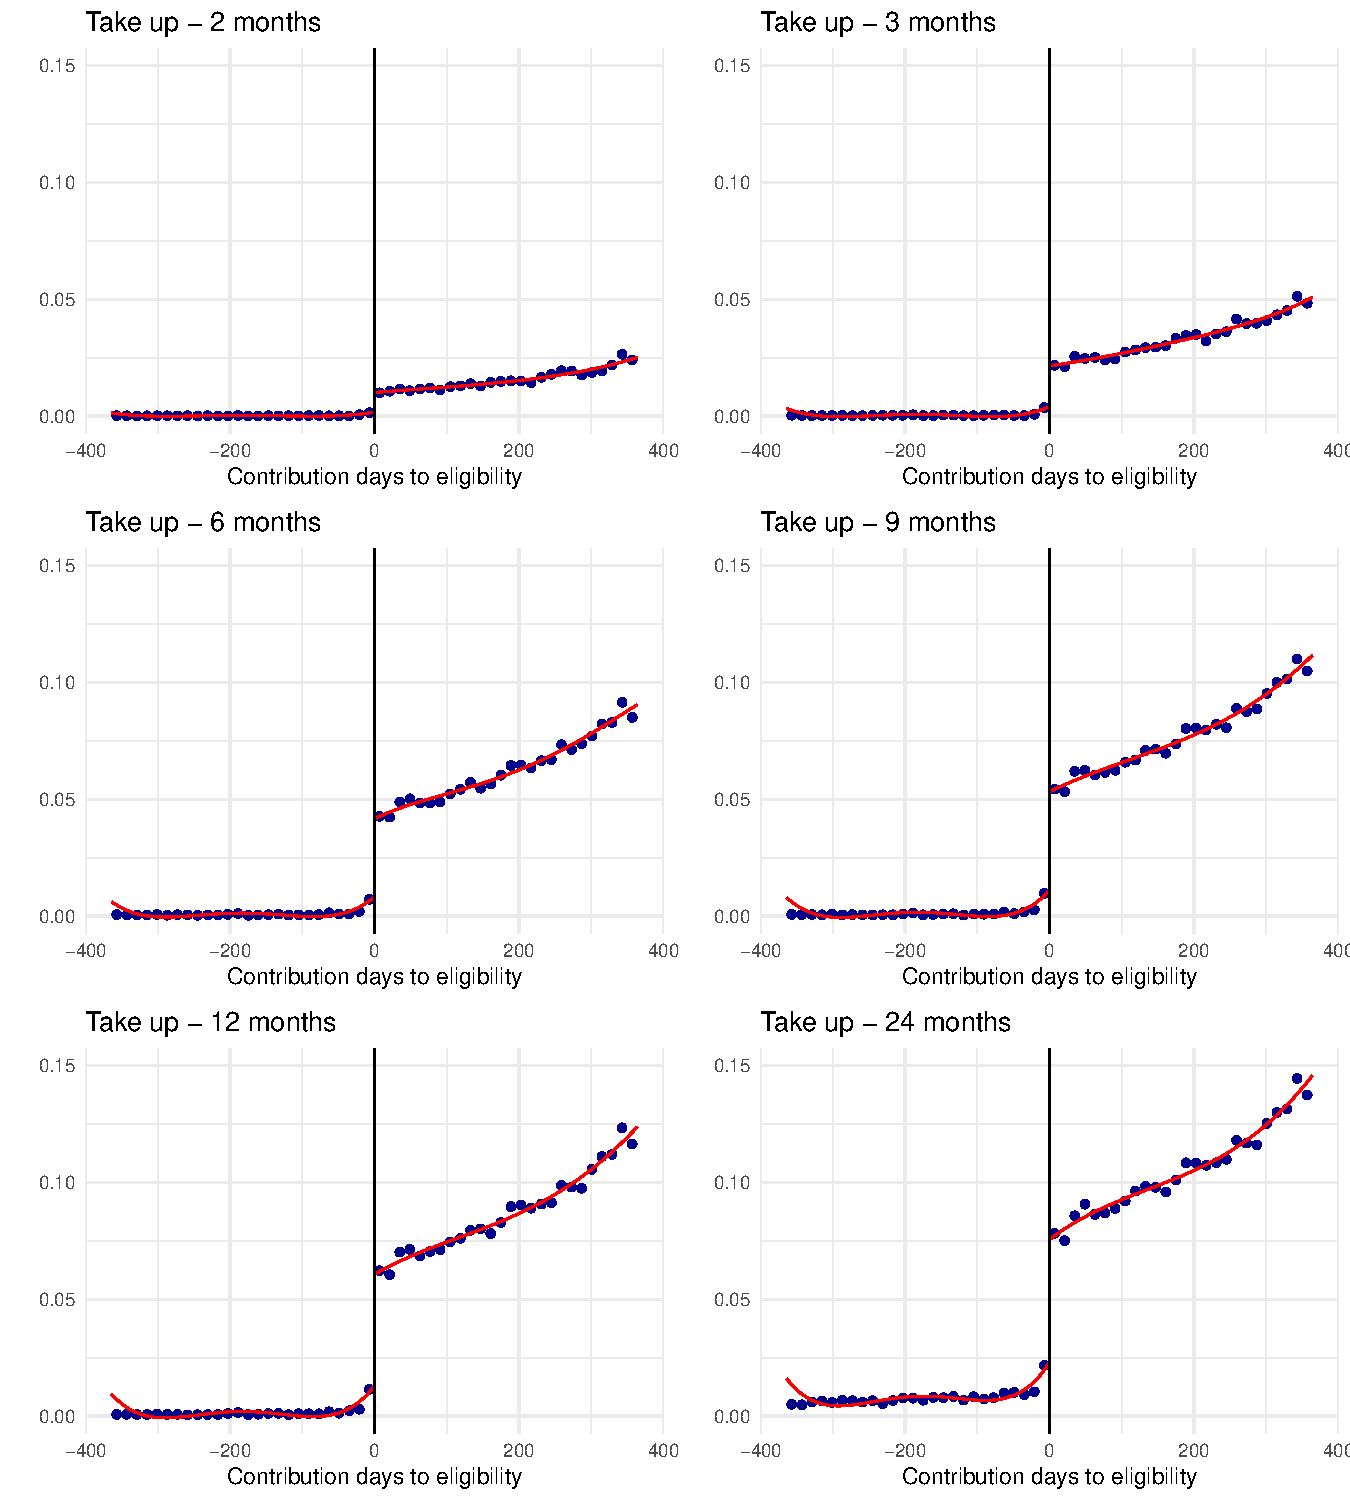
\includegraphics[keepaspectratio]{thesis_files/figure-pdf/unnamed-chunk-13-1.pdf}}

\emph{Note:} his figure shows (\emph{i}) sample means for evenly-spaced
14-day bins relative to the eligibility threshold, and (\emph{ii}) the
underlying regression function estimated using a triangular kernel,
optimal bandwidth and a linear local polynomial using Calonico,
Cattaneo, and Titiunik (\citeproc{ref-calonico2015}{2015}).

}

\end{figure}%

\begin{figure}

\caption{\label{fig-path}Dynamic Effect of Eligibility on Survival and
Duration of Unemployment}

\centering{

\pandocbounded{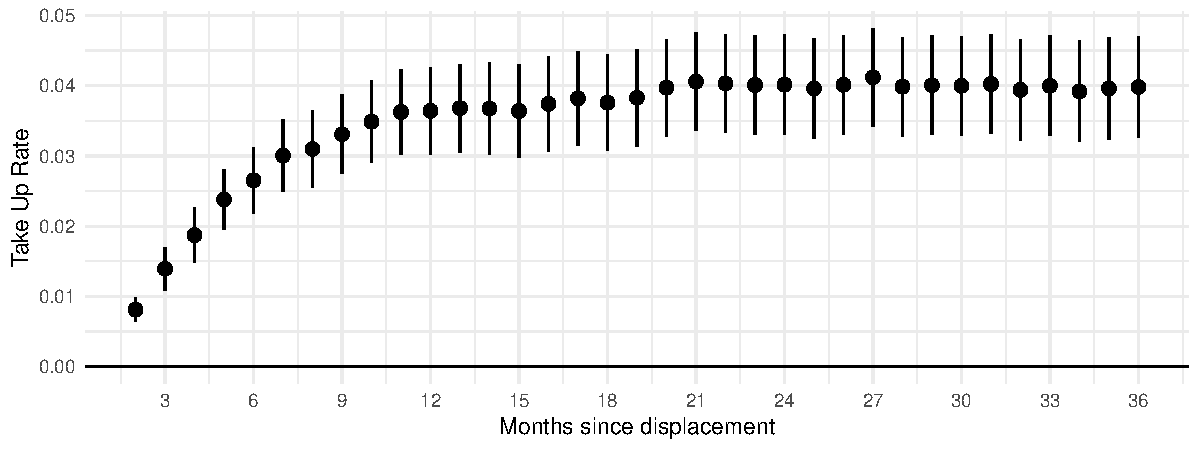
\includegraphics[keepaspectratio]{thesis_files/figure-pdf/unnamed-chunk-14-1.pdf}}

\emph{Note:} This figure shows the estimated coefficient of interest in
Equation~\ref{eq-1s} . The estimates are obtained using a triangular
kernel, optimal bandwidth and a linear local polynomial. Bias corrected
estimates and robust standard errors computed using Calonico, Cattaneo,
and Titiunik (\citeproc{ref-calonico2014}{2014}). 95 percent confidence
intervals.

}

\end{figure}%

\begin{table}

\caption{\label{tbl-job-search}Eligibility Effect: Job Search Outcomes}

\begin{minipage}{\linewidth}

\subcaption{\label{tbl-job-search-1}Survival and Duration of
Unemployment}

\centering{

\centering\centering
\resizebox{\ifdim\width>\linewidth\linewidth\else\width\fi}{!}{
\fontsize{8}{10}\selectfont
\begin{tabular}[t]{>{\raggedright\arraybackslash}p{11em}>{\centering\arraybackslash}p{8em}>{\centering\arraybackslash}p{8em}>{\centering\arraybackslash}p{8em}>{\centering\arraybackslash}p{8em}}
\toprule
  & Survival - 3 months & Survival - 36 months & Duration (wks) - 6 months & Duration (wks) - 36 months\\
\midrule
RPD & \num{0.007} & \num{0.001} & \num{0.085} & \num{0.648}\\
 & (\num{0.005}) & (\num{0.003}) & (\num{0.075}) & (\num{0.513})\\
\midrule
Mean at cutoff - ineligible & 0.78 & 0.108 & 20.5 & 51.9\\
Observations & 877,749 & 877,749 & 877,749 & 877,749\\
\bottomrule
\end{tabular}}

}

\end{minipage}%
\newline
\begin{minipage}{\linewidth}

\subcaption{\label{tbl-job-search-2}Next Job Quality}

\centering{

\centering\centering
\resizebox{\ifdim\width>\linewidth\linewidth\else\width\fi}{!}{
\fontsize{8}{10}\selectfont
\begin{threeparttable}
\begin{tabular}[t]{>{\raggedright\arraybackslash}p{11em}>{\centering\arraybackslash}p{8em}>{\centering\arraybackslash}p{8em}>{\centering\arraybackslash}p{8em}>{\centering\arraybackslash}p{8em}}
\toprule
  & Monthly earnings (2024 MXN) & Total earnings (2024 MXN) & Job duration (weeks) & Prev. job earnings\\
\midrule
RPD & \num{283.48} & \num{1469.40} & \num{0.56} & \num{276.07}\\
 & (\num{163.04}) & (\num{2178.74}) & (\num{0.62}) & (\num{215.71})\\
\midrule
Mean at cutoff - ineligible & 8,333 & 87,703 & 35.7 & 8,978\\
Observations & 873,434 & 873,434 & 873,434 & 873,434\\
\bottomrule
\end{tabular}
\begin{tablenotes}[para]
\item \textit{Note:} 
\item This table reports the estimated coefficient of interest from Equation 4.1, obtained using a local linear regression with a triangular kernel and optimal bandwidth selection. Bias-corrected point estimates and robust standard errors are computed following the procedure of Calonico, Cattaneo, and Titiunik (2014).
\end{tablenotes}
\end{threeparttable}}

}

\end{minipage}%

\end{table}%




\end{document}
